\chapter{Transport Methods} \label{Sec:transport}

The previous chapter covers the process of constructing a pointwise nuclear cross section library through the generation of a multigroup cross section library that accounts for resonance self-shielding effects. This library typically contains several tens or a few hundred energy groups, which is sufficient to capture the effects cross section variations, especially those from the nuclear resonances.

Only recently have full-core calculations using these fine energy-group libraries become feasible. That said, such calculations remain very computationally expensive and are still not practical for routine analyses. Instead, we go through a series of calculations. 

First, we perform detailed fine energy-group transport on the pin, unit cell level to obtain detailed flux profiles within the pin. These are typically done by solving the integral form of the transport equation with the collision probability method. 

Next, we perform a calculation on a lattice of fuel pins that accounts for coupling effects using the response matrix method. Then, we use the fluxes from the response matrices to perform energy condensation to collapse the fine energy-group library into a coarse group one with several to low tens of energy groups. 

Once we have this coarse group library, we then perform a transport calculation for an assembly or a collection of adjacent assemblies. Modern calculations typically use the method of characteristics, although other methods such as discrete ordinates are employed as well. 

Finally, we can then use this information to perform another group collapse to a few (often two or three) group cross section set and perform a full-core calculation using the nodal diffusion method.

This chapter covers the transport-based methods from the pin to the assembly level, leaving nodal diffusion to the following chapter. Here we discuss the collision probability method in the context of cylindrical fuel pins that are found in light-water reactors. For the assembly level, we cover the discrete ordinates method on a 2-D Cartesian grid. While the choice of discrete ordinates is not ideal for assembly-level calculations specifically, it is by far the most broadly used deterministic transport method and is extensively used in nuclear engineering applications.




%%%%%%%%%%%%%%%%%%%%%%%%%%%%%%%%%%%%%%%%%%%%%%%%%%%%%%%%%%%%%%%%%%%%%%%%%%%%%%%%%%%%%%%%%%%%%%%%%%%%
\section{Collision Probability Method}

In this section we derive the collision probability formulation of the transport equation, which serves the basis of the method for computing the scalar flux distribution within a fuel pin unit cell. Here we derive the integral transport equation and then formulate the collision probability equations in 1-D planar geometry and 2-D geometry. In the former case we can fully arrive at an analytical expression to completely remove any angular discretization. In 2-D, however, we apply a numerical ray tracing scheme.




\subsection{Integral Transport Equation}

The multigroup neutron transport equation assuming isotropic scattering can be written as
\begin{subequations}
\begin{align}
  \nabla \cdot \psi_g(\pos,\dir) + \Sigma_{t,g}(\pos) \psi_g(\pos,\dir) = \frac{1}{4\pi} q_g(\pos),
\end{align}
where the source $q_g$ contains isotropic scattering and fission:
\begin{align}
  q_g(\pos) = \sum_{g'=1}^G \Sigma_{s0,g' \rightarrow g}(\pos) \phi_{g'}(\pos) + \frac{1}{k} \chi_g \sum_{g'=1}^G \nu\Sigma_{fg'}(\pos) \phi_{g'}(\pos) .
\end{align}
We assume an isotropic angular flux on the boundary:
\begin{align}
  \psi(\pos,\dir) = \psi^b(\pos), \quad \pos \in \partial \Gamma, \quad \nhat \cdot \dir < 0 .
\end{align}
\end{subequations}

The assumption of isotropic scattering and boundary conditions is not strictly necessary for the integral transport equation, but is an important practical limitation of the collision probability method. To correct for this, we often replace the total cross section with the transport cross section (often with the inscatter method) and the within-group scattering cross section with the transport-corrected $P_0$ cross section. Whether or not this is done does not impact the results, only the numerical value of the cross sections, so we will just use the conventional nomenclature here.

We define the coordinate $s$ to be a spatial variable along the direction of flight $\dir$. The streaming operator can be recast as the directional derivative,
\begin{align}
  \dir \cdot \nabla 
  &= \Omega_x \dho{}{x} + \Omega_y \dho{}{y} + \Omega_z \dho{}{z} \nonumber \\
  &= \frac{dx}{ds} \dho{}{x} + \frac{dy}{ds} \dho{}{y} + \frac{dz}{ds} \dho{}{z} \nonumber \\
  &= \frac{d}{ds} ,
\end{align}
to obtain the characteristic form of the transport equation:
\begin{align}
  \frac{d}{ds} \psi(\pos,\dir) + \Sigma_t(\pos) \psi(\pos,\dir) = \frac{1}{4\pi} q(\pos),
\end{align}
Here we suppress the group indices since they are common on all terms.

This is a first-order ordinary differential equation along $s$ that be solved using the integrating factor:
\begin{align}
  I(s) = \exp\left[ \int_0^s \Sigma_t(s') ds' \right] = e^{-\tau(s)},
\end{align}
where $\tau$ is the optical distance from the beginning of the trajectory, typically the region boundary to point $s$. Applying the integrating factor and solving the transport equation gives
\begin{align}
  \psi(s) = \psi_b e^{-\tau(s)} + \frac{1}{4\pi} \int_0^s q(s') e^{-\tau(s-s')} ds' .
\end{align}
The first term is the angular flux from the boundary undergoing exponential attenuation a distance $s$. The second term is the contribution from the scattering plus fission source, where each interval $ds'$ contributes some number of neutrons to the angular flux at point $s$.

The conversion into the characteristic coordinate system is convenient for obtaining a solution in terms of an integral, but it is usually preferred to work in the global coordinate system. We can transform back into the global coordinates to obtain the integral form of the transport equation:
\begin{align}
  \psi(\pos,\dir) = \psi_b( \pos - s\dir ) e^{-\tau(\pos, \pos - s\dir )} + \frac{1}{4\pi} \int_0^{s(\pos,\dir)} q(\pos - s' \dir) e^{-\tau(\pos, \pos - s'\dir )} ds' \label{Eq:transport_integralFormAngularFlux}
\end{align}
Here $s$ is a the chord length and depends on the position $\pos$ and direction $\dir$ and the optical depth is
\begin{align}
  \tau(s) = \int_0^{s} \Sigma_t(\pos - s'\dir) ds' .
\end{align}

In principle, if we are given the cross sections and the source at all points in the domain, we can compute the angular flux at any point within the domain by evaluating the integral. In practice, this can only be done analytically for a very small number of cases and needs to be done numerically. That said, we can actually go one step further and find an integral equation for the scalar flux by integrating the equation over all directions. We can convert the first term for the boundary condition into a surface integral and the second term for the internal source into a volume integral. Leaving the details as an exercise, we quote the result as
\begin{align}
  \phi(\pos) 
  &= \int_{\partial\Gamma} \psi_b(\pos') e^{-\tau(\pos,\pos')} \frac{ \nhat' \cdot ( \pos' - \pos ) }{ | \pos - \pos' |^3 } dA' + \int_\Gamma \frac{q( \pos' ) }{4\pi | \pos - \pos' |^2 } e^{-\tau(\pos,\pos')} dV', \label{Eq:transport_integralFormScalarFlux}
\end{align}
where $\tau(\pos,\pos')$ is the optical distance between locations $\pos$ and $\pos'$ along a straight-line trajectory and $\nhat'$ denotes the outward unit normal at position $\pos'$.




\subsection{1-D Planar Geometry}

The simplest manifestation of the collision probability method is in 1-D planar or slab geometry. It turns out that in this coordinate system we can work out the problem analytically for the case where the source can be represented as a piecewise constant function such as in a numerical discretization scheme. The net effect is that while we are still required to perform a spatial discretization, we can completely remove the need for any angular discretization. Unfortunately, this result does not extend to two or three spatial dimensions, but, as we discuss in the next section, there are some simplifications that occur in 2-D geometry.

In 1-D planar geometry we demand that the material properties and sources are uniform out to infinity in the $y$ and $z$ directions, permitting spatial variation in the $x$ direction only. This symmetry not only removes two of the three spatial dimensions, but also removes the azimuthal variation of the angular flux, leaving only the directional dependence of the polar cosine $\mu$ with respect to the $x$ axis. Next we assume for simplicity that there is no boundary flux such that the first term in Eq.~\eqref{Eq:transport_integralFormScalarFlux} vanishes---this is not strictly necessary and it actually is not too difficult to include, but it does make the derivation less cluttered.

We then write the volume integral in Eq.~\eqref{Eq:transport_integralFormScalarFlux} in cylindrical coordinates about the $x$ axis:
\begin{align}
  \phi(x) 
  &= \int_{-\infty}^\infty \int_0^{2\pi} \int_0^\infty \frac{q( x' ) }{4\pi | \pos' - \pos |^2 } e^{-\tau(\pos,\pos')} r' dr' d\omega' dx'.
\end{align}
Here $r'$ is a radial coordinate from the origin situated at $x$, $\omega'$ is the polar angle about the $x$-axis, and $x'$ is the length along the $x$ axis.

Next, we define the ratio of the distance $| \pos' - \pos |$ to its projection upon the $x$-axis as
\begin{align}
  \rho = \frac{ | \pos' - \pos | }{ | x' - x | } .
\end{align}
We can then relate the optical distance $\tau(\pos,\pos')$ to the optical depth along the projection on the $x$-axis as
\begin{align}
  \tau(\pos,\pos') = \rho \tau(x,x') .
\end{align}
We can then relate the distance $| \pos' - \pos |$ to the radial coordinate $r'$ and the projection by noting they form a right triangle. This gives
\begin{align}
  | \pos' - \pos |^2 = ( r' )^2 + | x' - x |^2 .
\end{align}
Applying the ratio $\rho$ and solving for the radial variable we get
\begin{align}
  ( r' )^2 = ( \rho^2 - 1 ) | x' - x |^2 .
\end{align}

We can then perform a change of variables from $r'$ to $\rho$,
\begin{align}
  r' dr' = \rho | x' - x |^2  d\rho ,
\end{align}
and apply the ratio of optical depths to get an expression for the scalar flux of
\begin{align}
  \phi(x) 
  &= \int_{-\infty}^\infty \int_0^{2\pi} \int_1^\infty \frac{q( x' ) }{4\pi | \pos' - \pos |^2 } e^{-\rho \tau(x,x')} | x - x' |^2 \rho d\rho d\omega' dx'.
\end{align}
Evidently there is polar symmetry, so we can trivially integrate out the $\omega'$ coordinate. We can also apply the definition of $\rho$ to put $|\pos' - \pos|$ in terms of $|x' - x|$. We then get
\begin{align}
  \phi(x) 
  &= \frac{1}{2} \int_{-\infty}^\infty q(x') \int_1^\infty  \frac{e^{-\rho \tau(x,x')}}{\rho}  d\rho  dx'.
\end{align}

Here we are a bit stuck. Thankfully the integral over $\rho$ can be written as a special function known as the \emph{exponential integral} that is defined as
\begin{align}
  E_n(x) = \int_1^\infty \frac{ e^{-xt} }{ t^n } dt .
\end{align}
Applying the definition of the exponential integral allows us to ``carry out'' the $\rho$ integration to get
\begin{align}
  \phi(x) &= \frac{1}{2} \int_{-\infty}^\infty q(x') E_1[ \tau(x,x') ]  dx'. \label{Eq:transport_integralFormScalarFlux_1DPlanar}
\end{align}

Next we must specify the source distribution $q$. In the collision probability method we assume that the source is piecewise constant, which implies we make the flat source approximation on a discrete set of intervals. Suppose the spatial domain is finite and is subdivided into intervals where the source is approximated to be spatially constant. We define the centers of the intervals to have values $x_i$ with full-integer indices and the edges between them to have half-integer indices such that the material properties and sources are uniform between $x_{i-1/2} \le x < x_{i+1/2}$. We let $\phi_i$ be the volume-averaged scalar flux over the interval,
\begin{align}
  \phi_i = \frac{1}{\Delta x_i} \int_{x_{i-1/2}}^{x_{i+1/2}} \phi(x) dx,
\end{align}
where the mesh spacing $\Delta x_i = x_{i+1/2} - x_{i-1/2}$. 

We now integrate Eq.~\eqref{Eq:transport_integralFormScalarFlux_1DPlanar} for the scalar flux over the spatial domain:
\begin{align}
  \phi_i = \frac{1}{2 \Delta x_i} \int_{x_{i-1/2}}^{x_{i+1/2}} \sum_{i'} \int_{x_{i'-1/2}}^{x_{i'+1/2}} q_{i'} E_1[ \tau(x,x') ]  dx' dx.
\end{align}
Here the original integral from $-\infty$ to $\infty$ has been replaced with the sum of the integrals over each interval $i'$ and the source term $q(x') = q_{i'}$ in the interval containing $x_{i'}$.

We then define the first-flight collision probability $P_{ii'}$ as the probability a neutron born uniformly and isotropically within the spatial region containing $x_{i'}$ experiences its first collision within the spatial region containing $x_i$. This is the volume-averaged flux multiplied by the local total cross section,
\begin{align}
  P_{ii'} = \frac{ \Sigma_{t,i} }{ 2 \Delta x_i } \int_{x_{i-1/2}}^{x_{i+1/2}} \sum_{i'} \int_{x_{i'-1/2}}^{x_{i'+1/2}} E_1[ \tau(x,x') ]  dx' dx.
\end{align}
These two integrals can then be evaluated analytically. We have two cases, one for a neutron born and experiencing its first collision within the same element,
\begin{subequations}
\begin{align}
  P_{ii} = 1 - \frac{1}{2 \Sigma_{t,i} \Delta x_i} \left[ 1 - 2 E_3( \Sigma_{t,i} \Delta x_i ) \right] ,
\end{align}
and when the starting and final elements differ,
\begin{align}
  P_{ii'} = \frac{1}{2 \Sigma_{t,i} \Delta x_i} \left[ E_3( \tau_{ii'} ) - E_3( \tau_{ii'} + \tau_i ) - E_3( \tau_{ii'} + \tau_{i'} ) + E_3( \tau_{ii'} +  \tau_i +  \tau_{i'} ) \right] ,
\end{align}
\end{subequations}
where $\tau_i = \Sigma_{t,i} \Delta x_i$, the optical thickness along the $x$ axis of region $i$, and $\tau_{ii'}$ is the optical distance (along the $x$ axis) between regions $i$ and $i'$.

We can then write the volume-averaged collision rate in region $i$ in terms of the first-flight collision probability as
\begin{align}
  f_i = \Sigma_{t,i}  \phi_i \Delta x_i = \sum_{i'} P_{ii'}  q_{i'} \Delta x_{i'}.
\end{align}
The source term can be written as isotropic scattering and fission components:
\begin{align}
  q_{i} = \Sigma_{s,i} \phi_i + S_i,
\end{align}
where $S_i$ corresponds to the inscatter plus fission source in region $i$. We can then move the within-region scattering term to the left-hand side and then express the collision rates as the solution of a matrix-vector equation:
\begin{subequations}
\begin{align}
  \mathbf{H f} = \mathbf{s} ,
\end{align}
where the elements of the coefficient matrix and source vector are
\begin{align}
  H_{ii'}	&= \delta_{ii'} - \frac{\Sigma_{s,i'}}{\Sigma_{t,i'}} P_{ii'} , \\
  s_i  		&= \sum_{i'} P_{ii'} S_{i'} \Delta x_{i'} ,
\end{align}
\end{subequations}
where $\delta_{ii'}$ is the Kronecker delta function.

From here, we simply evaluate the $P_{ii'}$ given the optical thicknesses of each region and solve the linear system. The advantage of the collision probability method in planar geometry is that we do not require any angular discretization and can handle that dimension exactly. The disadvantage is that the use of the flat-source approximation means that the discretization error goes as $\Delta x$, which has a slower convergence rate than what is possible using other methods such as discrete ordinates. This means that for a geometrically large system, the number of spatial elements needs to be large, and size of matrices grows very quickly. Furthermore, the matrix $\mathbf{H}$ is dense meaning that the fast linear solvers for sparse matrices are of no use and we are stuck using slower dense linear solvers. 

This unfavorable geometric scaling is the reason why the collision probability method is used primarily for geometrically small systems, such as a fuel pin cell. In the case of a pin cell, there are often very steep flux gradients that would necessitate a very high-order angular discretization that the collision probability method obviates. And in these situations, the collision probability method is probably the fastest transport method available.





\subsection{2-D Geometry}

In the previous section we derive the equations for 1-D planar geometry. While this is useful for introducing the method, 1-D is unfortunately not applicable to the analysis of a fuel pin. At a minimum we need to work in two spatial dimensions where we assume the sources and material properties are uniform in the $z$ direction. For a conventional reactor, the active core region is extremely tall compared to the size of the fuel pin and treating the axial dimension as infinite to obtain the $x$-$y$ flux distribution within a pin is a very good approximation. 

Unfortunately, in 2-D we can only partial evaluate the integrals, namely the polar directional variable. Evaluating the remaining integrals necessitates the use of a numerical scheme, which is covered in the following section. Here we give the constituent integral equations that need to be solved.

In 2-D the problem has spatial variation along $x$ and $y$ and is infinite and uniform in $z$. The symmetry of the problem is such that the angular flux along a direction $\dir$ pointed above the $x$-$y$ plane is identical to the angular flux reflected below the plane. We are free to define the polar axis for the directional coordinate system $\dir$, and for the collision probability method we select this to be along $\zhat$. From this we can project all quantities out of the $x$-$y$ plane into it, which permits us to carry out the integration over the polar angle component of $\dir$.

We first define $\dir_p$ as a unit vector in the $x$-$y$ plane corresponding to the projection of the direction of flight unit vector $\dir$ out of the plane. We let $s(\pos,\dir)$ be the distance in 3-D space and $r$ be the distance projected onto the $x$-$y$ plane. Because the polar axis is along $z$, we have
\begin{align}
  r = s \sin\theta,
\end{align}
where $\theta$ is the polar angle. We can also relate the unit vectors $\dir$ (in 3-D) and $\dir_p$ (on the 2-D plane) by
\begin{align}
  ( \nhat \cdot \dir ) = ( \nhat \cdot \dir_p ) \sin\theta .
\end{align}
We can then assert that the isotropic boundary flux and internal source at any point are equivalent to their projection on the $x$-$y$ plane:
\begin{subequations}
\begin{align}
  \psi^b( \pos - s \dir ) &= \psi^b( \pos - r \dir_p ) , \\*
  q( \pos - s \dir ) &= q( \pos - r \dir_p ) .
\end{align}
\end{subequations}

We now return to the integral transport solution of the angular flux from Eq.~\eqref{Eq:transport_integralFormAngularFlux} and apply the projection onto the $x$-$y$ plane. We have
\begin{align}
  \psi(\pos,\dir) 
  &= \psi^b( \pos - r \dir_p ) \exp\left[ -\frac{\tau(\pos,\pos - r \dir_p)}{\sin\theta} \right] \nonumber \\
  &+ \int_0^{r(\pos,\dir_p)} \frac{q( \pos - r' \dir_p )}{4\pi \sin\theta } \exp\left[ -\frac{\tau(\pos,\pos - r' \dir_p)}{\sin\theta} \right] dr'.
\end{align}

Because the angular flux at the boundary is isotropic, it is often convenient to express it in terms of the inward partial current $J^-$. Solving for this we have
\begin{align}
  J^-(\pos - r \dir_p) 
  &= \int_{\dir \cdot \nhat < 0} | \dir \cdot \nhat |  \psi^b( \pos - r \dir_p ) d\Omega \nonumber \\*
  &= \psi^b( \pos - r \dir_p ) \int_{\dir \cdot \nhat < 0} | \dir \cdot \nhat | d\Omega  \nonumber \\*
  &= \pi \psi^b( \pos - r \dir_p ).
\end{align}
The boundary flux may be pulled out of the integral because it is assumed to be isotropic. It is important here to note that $\dir$ and $\dir_p$ are different variables and the equations for finding fluxes and currents are still integrated over the actual directions of flight $\dir$ and not the projected unit vector $\dir_p$. Therefore, the angular flux can then be written as
\begin{align}
  \psi(\pos,\dir) 
  &= \frac{1}{\pi} J^-(\pos - r \dir_p) \exp\left[ -\frac{\tau(\pos,\pos - r \dir_p)}{\sin\theta} \right] \nonumber \\
  &+ \int_0^{r(\pos,\dir_p)} \frac{q( \pos - r' \dir_p )}{4\pi \sin\theta } \exp\left[ -\frac{\tau(\pos,\pos - r' \dir_p)}{\sin\theta} \right] dr'.
\end{align}

The scalar flux can be found by integrating the angular flux over all directions of flight $\dir$ where the differential solid angle is again
\begin{align}
  d\Omega = \sin\theta d\theta d\gamma.
\end{align}
Recall the unit vector $\dir_p$ lies in the $x$-$y$ plane. The solid angle integrates over the entire unit sphere. Since here we let the polar axis be along $z$  the variable $\dir_p$ is independent of the polar angle $\theta$, but does depend upon the azimuthal angle $\gamma$. Likewise, the coordinate $r$ also depends on $\gamma$. Therefore we have
\begin{align}
  \phi(\pos) &= \frac{1}{2\pi} \int_0^{2\pi} 4 J^-(\pos - r \dir_p) \int_0^{\pi/2} \exp\left[ -\frac{\tau(\pos,\pos - r \dir_p)}{\sin\theta} \right] \sin\theta d\theta d\gamma \nonumber \\*
  &+ \frac{1}{2\pi} \int_0^{2\pi} \int_0^{r(\pos,\dir_p)} q( \pos - r' \dir_p ) \int_0^{\pi/2} \exp\left[ -\frac{\tau(\pos,\pos - r' \dir_p)}{\sin\theta} \right] d\theta dr' d\gamma.
\end{align}
Since both integrands over the polar angle are symmetric in $\theta$ about $\theta/2$, we write the integrals as twice the half range.

The reason for doing this is we now have to appeal to another special function to evaluate the integral over $\theta$. We have the \emph{Bickley-Nayler function} defined by
\begin{align}
  \kin_n(x) = \int_0^{\pi/2} e^{-x/\sin\omega}  \sin^{n-1}\omega \hspace{0.25em} d\omega , \quad n \ge 1. \nonumber
\end{align}
Introducing the Bickley-Nayler functions into the expression for the scalar flux, we obtain the result
\begin{align} \label{Eq:transport_scalarFlux_OpticalPathIntegrals}
  \phi(\pos) &= \frac{1}{2\pi} \int_0^{2\pi} 4 J^-(\pos - r \dir_p) \kin_2 \left[ \tau(\pos,\pos - r \dir_p) \right] d\gamma \nonumber \\*
  &+ \frac{1}{2\pi} \int_0^{2\pi} \int_0^{r(\pos,\dir_p)} q( \pos - r' \dir_p ) \kin_1 \left[ \tau(\pos,\pos - r \dir_p) \right] dr' d\gamma.
\end{align}

We would now need to know more information about the problem to actually proceed with evaluating the remaining integrals. In practice, this must be done numerically, and to facilitate a numerical scheme, we convert the integral over $\gamma$ in the first term into a line integral $L'$ over the boundary of the problem and the double integral of the second term into a an integral over 2-D regions $A'$. After doing this, we have
\begin{align}
  \phi(\pos) &= \frac{1}{2\pi} \int_L \nhat' \cdot \frac{( \pos' - \pos )}{|\pos - \pos'|^2} 4 J^-(\pos') \kin_2 [ \tau(\pos,\pos') ] dL' \nonumber \\
  &+ \frac{1}{2\pi} \int_S \frac{q( \pos' )}{ |\pos - \pos'| } \kin_1 [ \tau(\pos,\pos') ] dA'.
\end{align}

We can also similarly derive the outward partial current at the boundary. This can be expressed as integrals over optical paths using the Bickley-Nayler functions as
\begin{align} \label{Eq:transport_outwardPartialCurrent_OpticalPathIntegrals}
  J^+(\pos) &= \frac{1}{2\pi} \int_0^\pi ( \nhat \cdot \dir_p )  4J^-(\pos - r \dir_p) \kin_3 [ \tau(\pos,\pos - r' \dir_p) ] d\gamma \nonumber \\*
  &+ \frac{1}{2\pi} \int_0^\pi \int_0^{r(\pos,\dir_p)}  ( \nhat \cdot \dir_p ) q( \pos - r' \dir_p ) \kin_2 [ \tau(\pos,\pos - r' \dir_p) ] dr' d\gamma .
\end{align}
We can then convert these into line and area integrals:
\begin{align}
  J^+(\pos) &= \frac{1}{2\pi} \int_L \frac{[ \nhat \cdot (\pos - \pos') ][ \nhat' \cdot (\pos' - \pos) ]}{|\pos - \pos'|^3} 4J^-(\pos') \kin_3 [ \tau(\pos,\pos') ] dL' \nonumber \\*
  &+ \frac{1}{2\pi} \int_S \frac{ \nhat \cdot ( \pos - \pos') }{|\pos - \pos'|^2} q( \pos' ) \kin_2 [ \tau(\pos,\pos') ] dA'.
\end{align}

From here, as with planar geometry, we need to discretize the domain and apply the flat source approximation on each spatial element. The numerical method of choice involves ray tracing, which provides a great deal of flexibility for the discretization, e.g., we are not restricted to a regular grid. All we need to specify are 2-D spatial elements $i$ having respective areas $A_i$ and segments on the problem boundary $j$ with respective lengths $L_j$. After integrating the equation of the scalar flux over the spatial element $i$ and the outward partial current over the boundary segment $j$, we have
\begin{subequations} \label{Eq:transport_fluxCurrent_collisionProbabilities2D}
\begin{align}
  \Sigma_{t,i} \phi_i A_i 	&= \sum_{i'} P[ A_i \leftarrow A_{i'} ] q_{i'} A_{i'} + \sum_{j'} P[ A_i \leftarrow L_{j'} ] J^-_{i'} L_{j'} , \\*
  J_j^+ L_j 				&= \sum_{i'} P[ L_j \leftarrow A_{i'} ] q_{i'} A_{i'} + \sum_{j'} P[ L_j \leftarrow L_{j'} ] J^-_{i'} L_{j'} .  
\end{align}
\end{subequations}

Here we have four types of first-flight probabilities. The first is the probability that a neutron born uniformly and isotropically in region $i'$ experiences its first collision in region $i$,
\begin{subequations} \label{Eq:transport_collisionProbabilities2D_DoubleAreaLineIntegrals}
\begin{align}
  P[ A_i \leftarrow A_{i'} ] = \frac{ \Sigma_{t,i} }{ A_{i'} } \int_i \int_{i'} \frac{ \kin_1 [ \tau(\pos,\pos') ] }{ 2\pi | \pos - \pos' | } dA' dA ;
\end{align}
the second is the probability that a neutron emitted uniformly and with an isotropic flux (cosine source) on boundary segment $j'$ experiences its first collision in region $i$,
\begin{align}
  P[ A_i \leftarrow L_{j'} ] = \frac{ 4 \Sigma_{t,i} }{ L_{j'} } \int_i \int_{j'} \nhat' \cdot ( \pos' - \pos ) \frac{ \kin_2 [ \tau(\pos,\pos') ] }{ 2\pi | \pos' - \pos |^2 } dL' dA ;
\end{align}
the third is the probability that a neutron emitted uniformly and isotropically within region $i'$ crosses bounding segment $j$ before experiencing a collision,
\begin{align}
  P[ L_j \leftarrow A_{i'} ] = \frac{ 1 }{ A_{i'} } \int_j \int_{i'} \nhat \cdot ( \pos - \pos' ) \frac{ \kin_2 [ \tau(\pos,\pos') ] }{ 2\pi | \pos - \pos' |^2 } dL' dA ;
\end{align}
and finally the probability that a neutron emitted uniformly and with an isotropic flux (cosine source) on boundary segment $j'$  crosses bounding segment $j$ before experiencing a collision is
\begin{align}
  P[ L_j \leftarrow L_{j'} ] = \frac{ 4 }{ L_{j'} } \int_j \int_{j'} [ \nhat \cdot ( \pos - \pos' ) ] [ \nhat' \cdot ( \pos' - \pos ) ] \frac{ \kin_3 [ \tau(\pos,\pos') ] }{ 2\pi | \pos' - \pos |^3 } dL' dL .
\end{align}
\end{subequations}

At this point we need to numerically integrate these equations to determine the first-flight probabilities. We can then form a linear system as with the 1-D case and solve for the collision rates and region fluxes. We next discuss the numerical ray tracing scheme that is used to numerically integrate Eqs.~\eqref{Eq:transport_collisionProbabilities2D_DoubleAreaLineIntegrals}.




\subsection{Ray-Tracing Method}

We now develop the ray-tracing method that is used to evaluate Eqs.~\eqref{Eq:transport_collisionProbabilities2D_DoubleAreaLineIntegrals}. Investigating these equations, they involve surface and/or line integrals, which means they range from two to four nested integrals that need to be calculated. While one could in principle apply any quadrature scheme, it turns out ray tracing allows us to effectively reduce the dimensionality of all the equations down to two integrals. Furthermore, in the next section we apply this to cylindrical geometry for a unit cell where symmetry permits a reduction to a single integral.

The idea of the ray-tracing method is to take the discretized problem where uniform material properties and sources are assumed within each region and further subdivide the problem using a set of parallel rays oriented along a particular direction. We can then use ray tracing to numerically evaluate the integrals along each parallel subinterval. Once this is done, we repeat the subdivision by picking a new set of parallel rays with a different orientation. We repeat the process for different parallel-ray orientations until we sweep out the entire azimuthal domain.

To obtain the equations for this, we begin with Eqs.~\eqref{Eq:transport_scalarFlux_OpticalPathIntegrals} and~\eqref{Eq:transport_outwardPartialCurrent_OpticalPathIntegrals} for the scalar fluxes and outward partial currents in terms of the path integrals. We integrate the scalar flux equation over spatial region $i$ and multiply by the total cross section and integrate the outward partial current equation over boundary segment $j$. This results in
\begin{subequations} \label{Eq:transport_collisionProbabilityMethod2D_collisionRate_outwardCurrent}
\begin{align}
   \phi(\pos) &= \frac{1}{2\pi} \sum_{j'} \Sigma_{t,i} \int_i \int_{j'} 4 J^-_{j'} \kin_2 \left[ \tau(\pos,\pos - r \dir_p) \right] d\gamma dA \nonumber \\*
  &+ \frac{1}{2\pi} \sum_{i'} \Sigma_{t,i} \int_i \int_{i'} \int_{r_1}^{r_2} q_{i'} \kin_1 \left[ \tau(\pos,\pos - r \dir_p) \right] dr' d\gamma dA, \\
  J^+(\pos) &= \frac{1}{2\pi} \sum_{j'} \int_j \int_{j'} ( \nhat \cdot \dir_p )  4J^-_{j'} \kin_3 [ \tau(\pos,\pos - r' \dir_p) ] d\gamma dL \nonumber \\*
  &+ \frac{1}{2\pi} \sum_{i'} \int_j \int_{i'} \int_{r_1}^{r_2}  ( \nhat \cdot \dir_p ) q_{i'} \kin_2 [ \tau(\pos,\pos - r' \dir_p) ] dr' d\gamma dL.  
\end{align}
\end{subequations}
Here the integration over the $r'$ is just over the segment within region $A_i$ or the one adjacent to the boundary segment $L_j$ for azimuthal inclination $\gamma$. The range of azimuthal angles is taken not over all angles, but rather just the range subtended by $A_i$ or $L_j$. Inspecting Eq.~\eqref{Eq:transport_fluxCurrent_collisionProbabilities2D}, the collision probabilities can be inferred to be
\begin{subequations}
\begin{align}
   P[ A_i \leftarrow A_{i'} ] &= \frac{ \Sigma_{t,i} }{ 2\pi A_{i'} } \int_i \int_{i'} \int_{r_1}^{r_2} \kin_1 \left[ \tau(\pos,\pos - r \dir_p) \right] dr' d\gamma dA , \\
   P[ A_i \leftarrow L_{j'} ] &= \frac{ 4 \Sigma_{t,i} }{ 2\pi L_{j'} } \int_i \int_{j'} \kin_2 \left[ \tau(\pos,\pos - r \dir_p) \right] d\gamma dA , \\
   P[ L_j \leftarrow A_{i'} ] &= \frac{ 1 }{ 2\pi A_{i'} } \int_j \int_{i'} \int_{r_1}^{r_2}  ( \nhat \cdot \dir_p ) \kin_2 [ \tau(\pos,\pos - r' \dir_p) ] dr' d\gamma dL, \\
   P[ L_j \leftarrow L_{j'} ] &= \frac{ 4 }{ 2\pi L_{j'} } \int_j \int_{j'} ( \nhat \cdot \dir_p ) \kin_3 [ \tau(\pos,\pos - r' \dir_p) ] d\gamma dL .
\end{align}
\end{subequations}

We can carry out the integration over the segment $r'$. We note the optical depth can be expended as
\begin{align}
  \tau( \pos, \pos - r' \dir_p ) = \tau( \pos, \pos - r_1 \dir_p ) + \Sigma_{t,i'} ( r' - r_1 ) . 
\end{align}
Since the cross section is constant over the segment, we can carry out the integral over the Bickley-Nayler function. We have for the region-to-region and region-to-edge probabilities,
\begin{subequations}
\begin{align}
  P[ A_i \leftarrow A_{i'} ] &= \frac{ \Sigma_{t,i} }{ 2\pi \Sigma_{t,i'} A_{i'} } \int_{i'} \int_i \kin_2 \left[ \tau(\pos,\pos - r_1 \dir_p) \right] - \kin_2 \left[ \tau(\pos,\pos - r_2 \dir_p) \right] dA d\gamma , \\
  P[ L_j \leftarrow A_{i'} ] &= \frac{ 1 }{ 2\pi \Sigma_{t,i'} A_{i'} } \int_{i'} \int_j ( \nhat \cdot \dir_p ) \nonumber \\*
  &\hspace{2cm} \times \left\{ \kin_3 \left[ \tau(\pos,\pos - r_1 \dir_p) \right] - \kin_3 \left[ \tau(\pos,\pos - r_2 \dir_p) \right] \right\} dL d\gamma .
\end{align}
\end{subequations}

Next, we do a transformation so that we rotate into a convenient coordinate system about a ray, defining
\begin{subequations}
\begin{align}
  \xi 	&=  x \cos\gamma + y \sin\gamma , \\
  \zeta &= -x \sin\gamma + y \cos\gamma .
\end{align}
\end{subequations}
Here $\xi$ is taken to be parallel to the ray defined by $\gamma$ and $\zeta$ is taken to be normal to it. The integral over the differential area and line elements are then
\begin{subequations}
\begin{align}
  \int_i dA &= \int_{\zeta_i^-}^{\zeta_i^+} \int_{\xi_i^-}^{\xi_i^+} d\xi d\zeta, \\
  \int_j dL &= \int_{\zeta_j^-}^{\zeta_j^+} d\zeta .
\end{align}
\end{subequations}
Here the $-$ and $+$ superscripts denote the respective entry and exit points of the ray into the element.

The region-to-region first-flight collision probability is then
\begin{align}
  P[ A_i \leftarrow A_{i'} ] &= \frac{ \Sigma_{t,i} }{ 2\pi \Sigma_{t,i'} A_{i'} } \int_{i'}  \int_{\zeta_i^-}^{\zeta_i^+} \int_{\xi_i^-}^{\xi_i^+} \bigg\{ \kin_2 \left[ \tau(\pos,\pos - r_1 \dir_p) \right] \nonumber \\*
  &\hspace{4.5cm} - \kin_2 \left[ \tau(\pos,\pos - r_2 \dir_p) \right] \bigg\} d\xi d\zeta d\gamma .
\end{align}
Because $\xi$ is aligned parallel to ray, we can carry out this integral analytically. We need to consider two cases, one where the neutron begins and collides in the same element $i$ and the case where they differ. These are
\begin{subequations} \label{Eq:transport_collisionProbabilities2D_rayTracing}
\begin{align}
  P[ A_i \leftarrow A_i ] 		&= 1 - \frac{ 1 }{ 2\pi \Sigma_{t,i'} A_{i'} } \int_0^{2\pi} \int_{\zeta_i^-}^{\zeta_i^+} \left[ \frac{\pi}{4} - \kin_3( \tau_i ) \right] d\zeta d\gamma , \\
  P[ A_i \leftarrow A_{i'} ] 	&= \frac{ 1 }{ 2\pi \Sigma_{t,i'} A_{i'} }  \int_0^{2\pi} \int_{\zeta_i^-}^{\zeta_i^+} \bigg[ \kin_3(\tau_{ii'}) - \kin_3(\tau_i + \tau_{ii'} ) - \kin_3(\tau_{ii'} + \tau_{i'}) \nonumber \\*
  &\hspace{3.8cm} + \kin_3( \tau_{ii'} + \tau_i + \tau_{i'} ) \bigg] d\zeta d\gamma , \quad i \ne i' .
\end{align}
The remaining first-flight probabilities are
\begin{align}
  P[ A_i \leftarrow L_{j'} ] &= \frac{4}{ 2\pi L_{j'} } \int_0^{2\pi} \int_{\zeta_i^-}^{\zeta_i^+} \left[ \kin_3(\tau_{ij'}) - \kin_3(\tau_{ij'} + \tau_i) \right] d\zeta d\gamma, \\
  P[ L_j \leftarrow A_{i'} ] &= \frac{ 1 }{ 2\pi \Sigma_{t,i'} A_{i'} } \int_0^{2\pi} \int_{\zeta_j^-}^{\zeta_j^+} \left[ \kin_3(\tau_{ji'}) - \kin_3(\tau_{ji'} + \tau_{i'}) \right] d\zeta d\gamma, \\
  P[ L_j \leftarrow A_{i'} ] &= \frac{ 2 }{ 2\pi L_{j'} }  \int_0^{2\pi} \int_{\zeta_j^-}^{\zeta_j^+} \kin_3( \tau_{ij'} ) d\zeta d\gamma.
\end{align}
\end{subequations}
Here we extended the domain of the azimuthal integration to the full range $[0,2\pi)$ with the understanding that if for given a value of $\gamma$ there is no ray subtended by the adjoining elements then the range of the $\zeta$ integration is zero.

As with 1-D planar geometry, we represent the collision rates in a column vector $\mathbf{f}$ where the $i$th element is now
\begin{subequations}
\begin{align}
  f_i = \Sigma_{t,i} \phi_i A_i .
\end{align}
We also have column vectors for the partial currents $\mathbf{j}^-$ and $\mathbf{j}^+$ with elements defined as
\begin{align}
  \mathbf{j}_j^\pm &= J_j^\pm L_j,
\end{align}
and the inscatter plus fission source vector $\mathbf{s}$ with elements
\begin{align}
  s_i = S_i A_i .
\end{align}
It is also conventional to define a diagonal scattering matrix $\mathbf{C}$ having elements
\begin{align}
  C_{ii'} = \delta_{ii'} \frac{ \Sigma_{s,i',g \rightarrow g} }{ \Sigma_{t,i'} } .
\end{align}
\end{subequations}
Here we explicitly included the group indices to note this is the \emph{within group} scattering cross section. From these definitions we can write the emission density vector
\begin{align}
  \mathbf{q} = \mathbf{Cf} + \mathbf{s} .
\end{align}

We then can define the various collision probabilities as matrices $\mathbf{P}_{AA}$, $\mathbf{P}_{AL}$, $\mathbf{P}_{LA}$, $\mathbf{P}_{LL}$, where the elements correspond to the region-to-region, boundary-to-region, region-to-boundary, and boundary-to-boundary probabilities in Eqs.~\eqref{Eq:transport_collisionProbabilities2D_rayTracing}. Given this, we write Eqs.~\eqref{Eq:transport_collisionProbabilityMethod2D_collisionRate_outwardCurrent} in matrix-vector form as
\begin{subequations} 
\begin{align}
  \mathbf{f}   &= \mathbf{P}_{AA} \mathbf{q} + \mathbf{P}_{AL} \mathbf{j}^- , \\
  \mathbf{j}^+ &= \mathbf{P}_{LA} \mathbf{q} + \mathbf{P}_{LL} \mathbf{j}^-
\end{align}
\end{subequations}

To close this linear system we require boundary conditions give values for elements of the inward partial current vector $\mathbf{j}^-$ or relate them to the outward partial currents $\mathbf{j}^+$. The two simplest cases are the vacuum boundary where $j_j^- = 0$ and the reflecting boundary where $j_j^- = j_j^+$. Suppose can define a diagonal albedo matrix $\mathbf{B}$ giving the relation between the partial currents as
\begin{align}
  \mathbf{j}^- = \mathbf{B j}^+
\end{align}
Then we can substitute in this along with the emission density and rearrange to put the inscatter plus fission sources on the right-hand side. We can then write this as a single linear system of equations
\begin{align} \label{Eq:transport_collisionProbabilityMethod2D_matrixVectorEquations}
  \left[ \begin{array}{c c}
  \mathbf{I} - \mathbf{P}_{AA} \mathbf{C} 	& - \mathbf{P}_{AL} \mathbf{B} \\
  -\mathbf{P}_{LA} \mathbf{C}				& \mathbf{I} - \mathbf{P}_{LL} \mathbf{B} \\ \end{array} \right]
  \left[ \begin{array}{c} \mathbf{f} \\ \mathbf{j}^+ \\ \end{array} \right] =
  \left[ \begin{array}{c} \mathbf{P}_{AA} \mathbf{s} \\ \mathbf{P}_{LA} \mathbf{s} \\ \end{array} \right] .
\end{align}
This linear system can then be solved for the collision rates and outward partial currents.

%\begin{subequations}
%\begin{align}
%  \mathbf{f}   &= \mathbf{P}_{AA} ( \mathbf{Cf} + \mathbf{s} )  + \mathbf{P}_{AL} \mathbf{B} \mathbf{j}^+ , \\
%  \mathbf{j}^+ &= \mathbf{P}_{LA} ( \mathbf{Cf} + \mathbf{s} )  + \mathbf{P}_{LL} \mathbf{B} \mathbf{j}^+
%\end{align}
%\end{subequations}




\subsection{Optical Reciprocity Relationships}

The calculation of the probability matrices $\mathbf{P}_{XY}$ require the computation of a large number of elements, i.e., the square or product of the number of regions or boundary segments. It turns out we can cut the number of computations roughly in half by applying the reciprocity relations. We can compute either the upper or lower triangular part of the matrix and use the reciprocity relations to obtain the other.

These apply the general reciprocity relation from transport theory given in Eq.~\eqref{Eq:thermalization_generalizedReciprocityTheorem}. By selecting the appropriate transport problems, we can obtain the following results:
\begin{subequations}
\begin{align}
  P[ A_i \leftarrow A_{i'} ] \Sigma_{t,i'} A_{i'} &= P[ A_{i'} \leftarrow A_{i} ] \Sigma_{t,i} A_{i} , \label{Eq:transport_reciprocityRelation_region_region} \\
  P[ A_i \leftarrow L_{j'} ] \frac{L_{j'}}{4} &= P[ L_{j'} \leftarrow A_{i} ] \Sigma_{t,i} A_{i} , \label{Eq:transport_reciprocityRelation_region_segment}  \\
  P[ L_j \leftarrow L_{j'} ] L_{j'} &= P[ L_{j'} \leftarrow L_{j} ] L_j .  \label{Eq:transport_reciprocityRelation_segment_segment}
\end{align}
\end{subequations}
Note that the first result is a generalization of Eq.~\eqref{Eq:thermalization_firstFlightCollisionReciprocityRelationship}.





%%%%%%%%%%%%%%%%%%%%%%%%%%%%%%%%%%%%%%%%%%%%%%%%%%%%%%%%%%%%%%%%%%%%%%%%%%%%%%%%%%%%%%%%%%%%%%%%%%%%
\section{Unit Cell Calculations}

The collision probability method is often applied to solve the transport problem on a representative unit cell. Because of the physics of the problem, we can cylindricize square or hexagonal lattice unit cells to reduce the number of integrals from two to one. We first cover this cylindricization process. We then show how the collision probability method
is applied to this simplified case for a single energy group. We then cover how different energy groups are coupled through scattering and the normalization of the fission source.




\subsection{Equivalent Cylindrical Unit Cell}

The collision probability method developed in the previous section can be applied directly to any 2-D geometry by numerically evaluating the collision probabilities using a series of rays for each azimuthal inclination. The fuel in conventional reactor is cylindrical in a square or hexagonal lattice arrangement. It turns out we can replace the square or hexagonal boundary with a cylindrical one, provided we appropriately treat the boundary condition---more on this shortly. This cylindrical unit cell allows us to apply symmetry and parametrically express the azimuthal inclination angle in terms of the location of the ray subdividing the unit cell.

The most common method is to replace the moderator region with a cylindrical equivalent where we preserve the volume of the moderator between the actual and cylindricized unit cells. This cylindrical unit cell is called a \emph{Wigner-Seitz equivalent cell}.

As we mentioned, the boundary condition needs to be treated correctly. In the actual unit cell, we typically use either reflecting or periodic boundary conditions as appropriate to capture the symmetry of the lattice. In the case of a reflecting boundary conditions the local inward partial current $J^-$ equals the computed outward partial current $J^+$. Using this boundary condition on a cylindricized cell leads to a trajectory near tangent to the cylindrical surface reflecting off the boundary a large number of times, which causes a significant overestimation of the scalar flux distribution in the outer moderator regions and unacceptably large errors throughout the unit cell.

This effect can be ameliorated by replacing the reflecting boundary on the unit cell edge with what is referred to as a \emph{white boundary condition}. With this new boundary condition, a neutron striking the boundary of the unit cell re-emerges with an isotropic angular flux (cosine source) distribution rather than at the reflection angle. While replacing the reflecting boundary condition with a white boundary condition is a bit ad hoc, but it turns out this is much more accurate.

Another problem arises with the collision probability method applied to a unit cell. When the cell contains a standard fuel pin, the neutron source is driven by the fission spectrum. Unfortunately for the purpose of the analysis, reactors have unit cells that do not contain fuel, i.e., those with water holes or control elements. Furthermore, some fuel elements contain strong burnable absorber nuclides that significantly suppresses the amount of fission throughout the pin by way of their high thermal neutron absorption cross section. As such we have little or no source driving the neutron distribution.


\begin{figure}[tb!]
\begin{center}

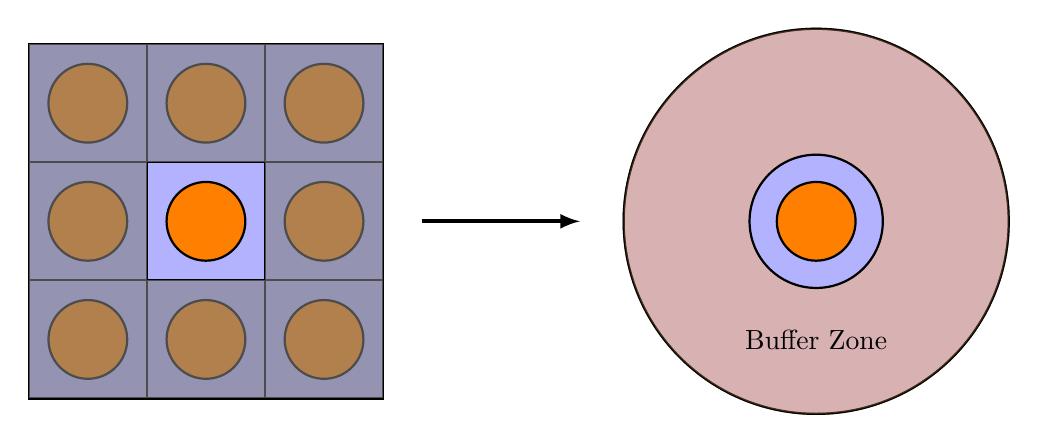
\begin{tikzpicture}

\filldraw[thick,fill=blue!30] (0,0) -- (4.5,0) -- (4.5,4.5) -- (0,4.5) -- cycle;
%\node at (0,-0.5*\h*\a+0.25) {$L$};

\foreach \i in {0,1.5,3} {
  \draw[thick] (0,\i) -- (4.5,\i);
  \draw[thick] (\i,0) -- (\i,4.5);
}

\foreach \i in {0,1.5,3} {
  \foreach \j in {0,1.5,3} {
    \filldraw[thick,fill=orange] ({\i+0.75},{\j+0.75}) circle (0.5cm);
  }
}

\fill[gray,opacity=0.6] (0,0) -- (4.5,0) -- (4.5,1.5) -- (0,1.5) -- cycle;
\fill[gray,opacity=0.6] (0,1.5) -- (1.5,1.5) -- (1.5,3) -- (0,3) -- cycle;
\fill[gray,opacity=0.6] (3,1.5) -- (4.5,1.5) -- (4.5,3) -- (3,3) -- cycle;
\fill[gray,opacity=0.6] (0,3) -- (4.5,3) -- (4.5,4.5) -- (0,4.5) -- cycle;


\draw[-latex, line width=0.5mm] (5,2.25) -- (7,2.25);

\filldraw[thick,fill=blue!30] (10,2.25) circle (2.4453cm);
\filldraw[thick,fill=orange!60,opacity=0.5] (10,2.25) circle (2.4453cm);
%\filldraw[thick,fill=gray!60,opacity=0.6] (10,2.25) circle (2.4453cm);
\filldraw[thick,fill=blue!30] (10,2.25) circle (0.8463cm);
\filldraw[thick,fill=orange]  (10,2.25) circle (0.5cm);

\node at (10,0.75) {Buffer Zone}; 

\end{tikzpicture}

\caption{Cylindrical unit fuel cell with buffer zone containing surrounding representative unit fuel cells.}
\label{Fig:neutronics_cylindicalFuelCell_Buffer}
\end{center}
\end{figure}


The resolution to this is we include what is called the \emph{buffer zone} surrounding the cylindrical unit cell containing a homogenized mixture of fuel, cladding, and moderator, but excluding any strong thermal absorbers. Typically the buffer zone has an cylindrical equivalent volume of (for a square lattice) the surrounding eight unit cells and contains a mixture that is homogenized by volume. The equivalent cylindrical unit cell with buffer zone is depicted in Fig.~\ref{Fig:neutronics_cylindicalFuelCell_Buffer}.

To have consistency between the fuel elements and simplify the numerical method, we surround \emph{all} unit cells, whether they be normal fuel, fuel containing burnable absorbers, water holes, control elements, etc. We then include a fixed internal source within only the buffer region with an intensity proportional to the energy group fission spectrum $\chi_g$ and turn off fission throughout the cell and buffer, treating it as absorption with no neutron emission. This allows us to treat all fuel elements as a fixed source problem for non-multiplying media. Because the problem under consideration is geometrically small, the perturbation in the flux shape within the pin versus treating fission multiplication is rather minor.

One effect of adding the buffer zone is that it moves the white boundary condition further away from the unit cell under consideration. This reduces any impact of making an ad hoc approximation on the boundary condition.




\subsection{Discretization and Applications of Symmetry}

In the previous section we define the equivalent cylindrical unit cell with a buffer zone containing a homogenized mixtures of the surrounding fuel pins that drive the source. We must now subdivide this cylindrical geometry into radial zones and then select the spacing of rays to numerically evaluate the integrals. 

We first subdivide the buffer zone and unit cell into a series of annular elements. We are free to choose the spacing arbitrarily, but should pick a resolution fine enough so that the local flat-source approximation is valid. Typically a normal fuel element requires a modest number of spatial zones, although it may be beneficial to add a few extra near the fuel-clad interface to resolve resonance absorption effects. Fuel containing burnable absorbers in particular requires a fine radial discretization to accurately capture the flux gradients and to support downstream isotopic depletion calculations.

The next step is to choose a spacing of rays, but first we note that we can apply symmetry arguments to reduce the double integral over $\zeta$ and azimuthal angle $\gamma$ into a single integral. To see this, we can imagine a ray entering the cylindrical region on the outer boundary at an arbitrary location with a similarly arbitrary inward direction. We can apply a coordinate transformation to rotate the system such that in this rotated coordinate system the ray is aligned along the $x$-axis, but at a different entry point. Now we can consider another ray at a different position and direction chosen such that when we apply a rotation to point along the $x$ axis, we end up at the same location. 

Because of the cylindrical symmetry in the geometry, the optical properties are identical for these two rays and we can represent both original rays by simply casting a single ray aligned along the $x$-axis at the location of the transformed coordinate system. By extension, we can map a distribution of incident positions-directions to that same location, all having equivalent optical properties. Furthermore, we can always map any position-direction pair to a corresponding optical equivalent oriented along the $x$-axis. Therefore, we only need to trace a set of rays oriented along the $x$ direction to solve the entire problem for all directions. (If we did not have cylindrical symmetry, we would get different optical properties and this simplification would break down.)
 
We can take this another step further and note that the rays cast going one direction are the same as the other. So this removes half of the problem domain, cutting the computational effort in half. And we can even make one final simplification and put a reflecting boundary condition that exploits symmetry.

In the case where we only exploit half symmetry, the annular regions are not convex, so the collision probabilities in an annular region may need to account for the probability that neutrons collide before leaving the annular region moving further inward and the probability that the neutron goes through the entire interior region and collides after re-emerging in that annular region. Effectively we have contributions of the form $P[ A_i \leftarrow A_i ]$ and $P[ A_i \leftarrow A_{i'}]$ accounting for each respective term.

For the case that we exploit quarter symmetry, we now have only convex regions, but at the cost of adding a reflecting boundary condition at the midplane, which can be subdivided into multiple segments having lengths $L_j$. For the boundary condition matrix $\mathbf{B}$, segments on the reflecting midplane have diagonal elements equal to one such that $J_j^- = J_j^+$. and are zero for segments on the outer boundary such that $J^-_j = 0$. We then need to compute all four probability elements to solve for the collision rates and this makes the linear system much larger.

It turns out there is very expedient approach to treat the reentrant annular elements that we discuss in the next section, meaning we are not required to handle the boundary cases.

The final choice we need to make before we can begin calculating is to select a ray spacing itself. This choice influences the accuracy of the calculation with the obvious tradeoff being computational expense. There are two conventional choices. One is to apply a uniform ray spacing such that the distance between the midpoints between adjacent rays is given by a width $\Delta h$. The other is to use a Gauss-Legendre quadrature integration scheme where the rays correspond to the abscissa of the quadrature set. Regardless, there needs to be a fine enough resolution to accurately resolve any flux gradients.




\subsection{Ray-Tracing Calculation}

In the previous section, we covered the discretization of the equivalent cylindrical unit cell. We are now ready to actually perform the ray-tracing calculation on this simplified geometry to compute approximate first-flight collision probabilities on an annular unit cell. Here we treat this for a single energy group and assume a \emph{vacuum boundary condition}. In the next section we discuss how to use these vacuum-boundary condition results to obtain what is obtained for a white boundary condition. Here we solve the problem for a single energy group given a known inscatter and fission source. In a following section we go over how to couple the energy groups.

First, some preliminaries. We write the collision probability as
\begin{align}
  P_{ij} = P[ A_i \leftarrow A_j ] .
\end{align}
Here we use the index $j$ as opposed to $i'$ since we do not compute boundary elements. Next, we define the \emph{collision intensity} as
\begin{align}
  T_{ij} = \Sigma_{t,j} A_j P_{ij} .
\end{align}
Because of the optical reciprocity relationship, the collision intensity is a symmetric function:
\begin{align}
  \Sigma_{t,j} A_j P_{ij} = \Sigma_{t,i} A_i P_{ji}, \quad T_{ij} = T_{ji} .
\end{align}
For this reason we tend to perform calculation with the collision intensities as opposed to probabilities. Note that many references (quite confusingly) refer to the collision intensities as the collision probabilities, even though they are clearly not so in a conventional sense---having units of length in 2-D (area in 3-D) as opposed to being dimensionless and not being bounded by one.

Next, we let $x_j(y)$ be denote the position of intersection of a ray aligned along the $x$ direction with height $y$ of the $j$th annular zone. The optical distance between the $y$-axis ($x = 0$) and $x_j$ is then
\begin{align}
  \tau(0,x_j) = \Sigma_{t,1}  \sqrt{ R_1^2 - y^2 } +  \sum_{m=2}^j \Sigma_{t,m} \left[ \sqrt{ R_m^2 - y^2 } - \sqrt{ R_{m-1}^2 - y^2 } \right]
\end{align}
We then define the following optical distances:
\begin{align}
  \tau_{ij}^\pm &= \tau(0,x_i) \pm \tau(0,x_j) , \quad x_i \ge x_j .
\end{align}


\begin{figure}[tb!]
\begin{center}

\begin{tikzpicture}

\filldraw[thick,fill=white]   (6.25,0) arc (0:180:6.25cm);
\filldraw[thick,fill=blue!30] (5.5,0) arc (0:180:5.5cm);
\filldraw[thick,fill=white]   (4.25,0) arc (0:180:4.25cm);
\filldraw[thick,fill=red!30]  (3.5,0) arc (0:180:3.5cm);
\filldraw[thick,fill=white]   (2.5,0) arc (0:180:2.5cm);

\draw[latex'-latex'] (-7,0) -- (7.5,0);
\draw[-latex] ( 0,0) -- ( 0,7);
\node at (7.375,-0.15) {\scriptsize $x$};
\node at (-0.15,6.875) {\scriptsize $y$};

\node at ({3*cos(60)},{3*sin(60)}) {$A_j$};
\node at ({5*cos(60)},{5*sin(60)}) {$A_i$};

\draw[dashed] (-7,1) -- (7.5,1);
\draw[dashed] (-7,2) -- (7.5,2);
\draw[thick,latex'-latex'] (7.25,1) -- (7.25,2);
\node[fill=white] at (7.25,1.5) {\scriptsize $\Delta y_k$};

\draw[line width=0.5mm,latex'-latex',blue] (-7,1.5) -- (6.75,1.5);

\draw (-3.175,2.25) -- (-3.175,-1);
\node[fill=white] at (-3.175,-0.325) {\scriptsize $x_j$};

\draw (-5.275,2.25) -- (-5.275,-1.375);
\node[fill=white] at (-5.275,-0.325) {\scriptsize $x_i$};

\draw (3.175,2.25) -- (3.175,-1.375);

\draw[thick,latex'-latex'] (-5.275,-0.75) -- (-3.175,-0.75);
\draw[thick,latex'-latex'] (-5.275,-1.125) -- ( 3.175,-1.125);

\node[fill=white] at ({0.5*(-5.275 + -3.175)},-0.75)  {\scriptsize $\tau_{ij}^-$};
\node[fill=white] at ({0.5*(-5.275 +  3.175)},-1.125) {\scriptsize $\tau_{ij}^+$};

%\filldraw[thick,fill=white] (0,0) circle (5cm);
%\filldraw[thick,fill=blue!30] (0,0) circle ( 4.5cm);
%\filldraw[thick,fill=white] (0,0) circle ( 3.5cm);
%\filldraw[thick,fill=red!30] (0,0) circle ( 2.5cm);
%\filldraw[thick,fill=white] (0,0) circle ( 1.5cm);

 

\end{tikzpicture}

\caption{Depiction of annular geometry and representative ray for the collision probability method.}
\label{Fig:neutronics_collisionProbabilityMethodAnnularGeometry}
\end{center}
\end{figure}


Now we consider the scenario depicted in Fig.~\ref{Fig:neutronics_collisionProbabilityMethodAnnularGeometry}. Here we have a source region $A_j$ shaded in red and a \emph{different} collision destination region $A_i$ shaded in blue such that $i \ne j$. We consider neutrons emitted on the blue ray $k$ depicted between the segment $\Delta y_k$. Neutrons are emitted within $A_j$ along this ray either going in the positive $x$ or negative $x$ direction. The rightward directed neutrons can collide in the annular region of $A_i$ on the right, and the leftward neutrons on the left.

From Eq.~\eqref{Eq:transport_collisionProbabilities2D_rayTracing}, the collision intensity for the leftward-moving neutron is
\begin{align}
  T_{ij}^- 
  &= \int_0^{R_j} \kin_3[ \tau(x_j,x_{i-1}) ] - \kin_3[ \tau(x_j,x_{i-1}) + \tau(x_{j-1},x_j) ]  \nonumber \\*
  &- \kin_3[ \tau(x_j,x_{i-1}) + \tau(x_{i-1},x_i) ] + \kin_3[ \tau(x_j,x_{i-1}) + \tau(x_{j-1},x_j) + \tau(x_{i-1},x_i)  ] \, dy \nonumber \\
  &= \int_0^{R_j} \kin_3[ \tau(x_j,x_{i-1}) ] - \kin_3[ \tau(x_{j-1},x_{i-1})  ] - \kin_3[ \tau(x_j,x_i)  ] + \kin_3[ \tau(x_{j-1},x_i) ] \, dy \nonumber \\
  &= \int_0^{R_j} \kin_3( \tau_{i-1,j}^- ) - \kin_3( \tau_{i-1,j-1}^-  ) - \kin_3( \tau_{i,j}^- ) + \kin_3( \tau_{i,j-1}^- ) \, dy.
\end{align}
Similarly, for the rightward-moving neutron, we obtain
\begin{align}
  T_{ij}^+ &= \int_0^{R_j} \kin_3( \tau_{i-1,j-1}^+ ) - \kin_3(\tau_{i,j-1}^+) - \kin_3(\tau_{i-1,j}^+) + \kin_3(\tau_{i,j}^+) \, dy.
\end{align}
Recall that the optical depths $\tau$ are implicitly functions of the ray location $y$.

The total collision intensity $T_{ij}$ is twice the sum of these terms, with the doubling arising because of symmetry across the $x$ axis. After a bit of rearrangement, we arrive at the following result:
\begin{align}
  T_{ij} 
  &= 2 ( T_{ij}^+ + T_{ij}^- ) \nonumber \\
  &= 2 \bigg[ \int_0^{R_j} \kin_3( \tau_{i,j}^+) - \kin_3( \tau_{i,j}^-) \, dy + \int_0^{R_j}  \kin_3( \tau_{i-1,j-1}^+) - \kin_3( \tau_{i-1,j-1}^-) \, dy \nonumber \\
  &\hspace{0.5cm} + \int_0^{R_j} \kin_3( \tau_{i,j-1}^+) - \kin_3( \tau_{i,j-1}^-) \, dy + \int_0^{R_j} \kin_3( \tau_{i-1,j}^+) - \kin_3( \tau_{i-1,j}^-) \, dy \bigg] \nonumber \\
  &= 2 \left( F_{i,j} + F_{i-1,j-1} - F_{i,j-1} - F_{i-1,j} \right) , \quad i \ne j.
\end{align}
Here we define the function
\begin{align}
  F_{ij} = \int_0^{R_j} \kin_3( \tau_{i,j}^+) - \kin_3( \tau_{i,j}^-) \, dy,
\end{align}
satisfying the identities
\begin{subequations}
\begin{align}
  F_{ij}  &= F_{ji}, \\*
  F_{0,j} &= F_{i,0} = 0.
\end{align}
\end{subequations}

The previous result only applies for $i \ne j$, i.e., where the source and collision regions differ. We can work out the analogous result for $j = i$:
\begin{align}
  T_{jj} = \Sigma_{t,j} A_j + 2  \left( F_{j,j} + F_{j-1,j-1} - F_{j,j-1} - F_{j-1,j} \right) .
\end{align}
We can combine these two results compactly as
\begin{align}
  T_{ij} = \delta_{ij}  \Sigma_{t,j} A_j + 2 \left( F_{i,j} + F_{i-1,j-1} - F_{i,j-1} - F_{i-1,j} \right) .
\end{align}

The evaluation of the collision intensities $T_{ij}$, or collision probabilities $P_{ij}$, in annular geometry is essentially the computation of the function $F_{ij}$. An algorithm is the subdivide the upper half of the problem into intervals with a spacing $\Delta y_k$ with a ray located at location $y_k$ in the center of the interval, which is the case depicted in Fig.~\ref{Fig:neutronics_collisionProbabilityMethodAnnularGeometry}. (When computers were much slower, it was more important to base the intervals on more sophisticated quadrature rules with Gauss-Jacobi being the preferred choice for this problem.) The computation of $F_{ij}$ is then
\begin{align}
  F_{ij} \approx \sum_k \left[ \kin_3( \tau_{i,j}^+) - \kin_3( \tau_{i,j}^-) \right] \Delta y_k .
\end{align}

The algorithm requires three nested loops. The outer loop is over each ray $k$, the next loop is over all source elements $i$ that the $k$th ray intersects, and the inner loop is over all collision elements $j \ge i$.

%
%For each ray $r$, we compute the lengths of each segment from the exterior boundary to either the other boundary or the reflecting midplane. These can be done by solving the surface equations in Sec.~\ref{Sec:libraryGeneration_monteCarloRayTracing}, where the solutions for the planar and cylindrical surfaces are given by Eqs.~\eqref{Eq:libraryGeneration_distanceToSurfaces}. These distances should be stored since they will be used repeatedly for each energy group.
%
%Once these distances are known, we loop over each ray $r$ and compute the first-flight collision probabilities. These can be tabulated for each probability using
%\begin{subequations}
%\begin{align}
%  P[ A_i \leftarrow A_i ] 		&= 1 - \frac{ 1 }{ \Sigma_{t,i'} A_{i'} } \sum_r \left[ \frac{\pi}{4} - \kin_3( \tau_i ) \right] \Delta h_r , \nonumber \\
%  P[ A_i \leftarrow A_{i'} ] 	&= \frac{ 1 }{ \Sigma_{t,i'} A_{i'} }  \sum_r \bigg[ \kin_3(\tau_{ii'}) - \kin_3(\tau_i + \tau_{ii'} ) - \kin_3(\tau_{ii'} + \tau_{i'}) \nonumber \\*
%  &\hspace{3.8cm} + \kin_3( \tau_{ii'} + \tau_i + \tau_{i'} ) \bigg] \Delta h_r , \quad i \ne i' . \\
%  P[ A_i \leftarrow L_{j'} ] &= \frac{4}{ L_{j'} } \sum_r \left[ \kin_3(\tau_{ij'}) - \kin_3(\tau_{ij'} + \tau_i) \right] \Delta h_r , \\
%  P[ L_j \leftarrow A_{i'} ] &= \frac{ 1 }{ \Sigma_{t,i'} A_{i'} } \sum_r \left[ \kin_3(\tau_{ji'}) - \kin_3(\tau_{ji'} + \tau_{i'}) \right] \Delta h_r , \\
%  P[ L_j \leftarrow A_{i'} ] &= \frac{ 2 }{  L_{j'} }  \sum_m \kin_3( \tau_{ij'} ) \Delta h_r .
%\end{align}
%\end{subequations}
%Here the optical distances $\tau$ use the region group total cross sections and the precomputed segment lengths for ray $r$, which may be zero should the ray not intersect the region or cross the boundary segment resulting in a zero contribution to the sum. These expressions assume a spacing with a width $\Delta h_r$ about ray $r$. Note that the factor of $2\pi$ is absent from the denominator. This vanished because of the cylindrical symmetry of the problem.
%
%Note that if we are treating all boundaries as vacuum, then we need not compute any of the collision probabilities involving boundary segments if the goal is to obtain the collision rates.




\subsection{White Boundary Condition}

The first-flight probabilities collision computed in the previous section assume a vacuum boundary on the exterior surface. We then apply a method developed by Carlvik that uses these collision probabilities to obtain new ones that are for the white boundary condition. We define the reflection coefficient for spatial region $i$ as
\begin{align}
  R_j = \Sigma_{t,j} A_j - \sum_i T_{ij} .
\end{align}
The first-flight collision probability for a white boundary condition is given by
\begin{align}
  \widehat{T}_{ij} = T_{ij} + \dfrac{R_i R_j}{ \displaystyle\sum_k R_k } .
\end{align}
We use these white boundary condition collision intensities to compute the white collision probabilities
\begin{align}
  \widehat{P}_{ij} = \frac{ \widehat{T}_{ij} }{ \Sigma_{t,j} A_j } .
\end{align}
Because all neutrons that reach the boundary are reflected back in, the sum of the collision probabilities over the colliding elements should be unity:
\begin{align}
  \sum_i \widehat{P}_{ij} = 1.
\end{align}




\subsection{Computation of Fluxes}

We are now finally ready to apply Eq.~\eqref{Eq:transport_collisionProbabilityMethod2D_collisionRate_outwardCurrent} to solve for the region fluxes. Since we are assuming a vacuum boundary condition for the original calculation, the inward partial current $J^+ = 0$. The presence of the white boundary condition is handled by the correction of the collision probabilities. Given this vacuum boundary condition, we have a linear equation for the collision rates
\begin{align}
  \left( \mathbf{I} - \widehat{\mathbf{P}}_{AA} \mathbf{C} \right) \mathbf{f} = \widehat{\mathbf{P}}_{AA}\mathbf{s} .
\end{align}
This matrix may be easily inverted to obtain the collision rates. The region fluxes are then simply given by
\begin{align}
  \phi_i = \frac{ f_i }{ \Sigma_{t,i} A_i } .
\end{align}

\subsection{Energy-Group Coupling and Rebalance} \label{Sec:transport_collsionProbability_energyGroupCoupling}

The coupling between energy groups is because of the group-to-group scattering cross section $\Sigma_{s,g' \rightarrow g}$ and rolled into the internal group source $S_g$. The method for treating the coupling is fairly standard across numerical transport methods. The idea is to subdivide the energy groups into fast and thermal groups with the key distinction being the fast groups do not involve any upscattering whereas the thermal groups do. We define group $g_t$ as being the first thermal energy group.

The process begins by first looping over the fast groups in descending order, starting at the highest energy group. The internal source within a spatial zone is given by
\begin{align}
  S_{i,g} = \sum_{g'=1}^{g-1} \Sigma_{s,i,g' \rightarrow g} \phi_{i,g'} + \chi_{i,g} , \quad g < g_t.
\end{align}
Here $\chi_{i,g}$ is the group fission spectrum that is nonzero only within the buffer region. Once the source is computed for group $g$, we perform the collision probability method to estimate the collision rates and therefore determine the fixes. Because we are looping in descending group order, the group fluxes needed were already calculated earlier in the process.

Once we reach group the first thermal group $g_t$, we need to account for upscattering, which requires us to use the group fluxes that we have not yet calculated. This necessitates iterating over the thermal groups. Define the fluxes for $k$th iteration as having a superscript in parentheses. We must provide an initial guess of the thermal fluxes, where unity or zero are common choices, for iteration $k = 0$. The group source for the $k$th iteration is then
\begin{align}
  S_{i,g}^{(k)} = 
  \sum_{g'=1}^{g_t-1} \Sigma_{s,i,g' \rightarrow g} \phi_{i,g'} 
  + \sum_{g'=g_t}^{g-1} \Sigma_{s,i,g' \rightarrow g} \phi_{i,g'}^{(k)} +  \sum_{g'=g+1}^{G} \Sigma_{s,i,g' \rightarrow g} \phi_{i,g'}^{(k-1)} + \chi_{i,g}, \quad g \ge g_t .
\end{align}
The first term is the sum over the fast groups; these do not have an iteration index because these are known and therefore fixed. The second term are for thermal groups at higher energy groups than the current group $g$; these use the fluxes we just solved for on the current iteration. The third term are for thermal fluxes we have not yet solved on this iteration and use the thermal fluxes from the previous iteration.

Following each iteration we need to perform a rebalancing to ensure neutron conservation in the thermal groups. This is referred to as a \emph{fundamental mode rebalance}. The process is we compute the flux-area weighted homogenized group cross sections as
\begin{align}
  \overline{\Sigma}_{x,g} = \dfrac{ \displaystyle\sum_i \Sigma_{x,i,g} \phi_{i,g} A_i }{ \displaystyle\sum_i \phi_{i,g} A_i } 
\end{align}
The fluxes here are for the iteration that just concluded.

Next we obtain the spectrum $\overline{\phi}_g$ using the global neutron balance equation for each group:
\begin{align}
  ( \overline{\Sigma}_{t,g} - \overline{\Sigma}_{s,g \rightarrow g } ) \overline{\phi}_g = \sum_{g' \ne g } \overline{\Sigma}_{s,g' \rightarrow g } \overline{\phi}_{g'} + \chi_g .
\end{align}
The fluxes are then rebalanced using
\begin{align}
  \hat{\phi}_{i,g} = \phi_{i,g} \dfrac{ \overline{\phi}_g }{ \displaystyle\sum_i \phi_{i,g} A_i } .
\end{align}
This $\hat{\phi}$ is then set to the flux in the next iteration. We check convergence of the local group fluxes each iteration and see if they have converged within some user-defined tolerance.

Once we have convergence, the infinite multiplication factor for the fuel pin may be determined as
\begin{align}
  k_\infty = \dfrac{ \displaystyle\sum_g \overline{ \nu \Sigma }_{f,g} \overline{\phi}_g }{ \displaystyle\sum_g \overline{ \Sigma }_{a,g} \overline{\phi}_g } .
\end{align}





%%%%%%%%%%%%%%%%%%%%%%%%%%%%%%%%%%%%%%%%%%%%%%%%%%%%%%%%%%%%%%%%%%%%%%%%%%%%%%%%%%%%%%%%%%%%%%%%%%%%
\section{Cell Coupling and Energy Condensation}

In the previous section, we cover the method for computing the flux distribution on a single unit cell. In practice, we run such a calculation for each type of unit cell. This includes a calculation for each fuel pin for various enrichment and burnable absorber calculations and burnup as well as ones for each non-fuel containing unit cell, e.g., control elements or water holes.

The result of these calculations is a flux spectrum throughout the unit cell on a fine energy group structure, typically containing from several tens to a few hundred energy groups. The next step in the reactor analysis process is to run an assembly-level transport calculation, but this would be computationally expensive using this same energy fine group structure. Therefore, we use the results to condense the fine energy group cross sections onto coarse energy group structure, typically containing several to a few tens of energy groups.

The problem we run into is that we only ran calculations for each individual unit cell type independent of the others. In a real reactor, the flux spectrum of a unit cell is significantly influenced by the neighboring unit cells. Performing energy condensation without accounting for this effect would lead to significant errors in the coarse group cross sections and therefore negatively impact the quality of the downstream calculations.

Thankfully, there is a relatively simple approach to couple neighboring unit cells. This is done by performing low spatial fidelity 2-D transport calculations with the \emph{transmission probability method} on a coarse grid of (usually rectangular) homogenized regions within the full lattice. The result of these calculations are the outward partial currents that connect with the neighboring unit cells.

Once we have obtained these partial currents, the coupling between the unit cells is done using the \emph{response matrix method}. By solving the linear system of equations in the response matrix method, we can obtain the fine group fluxes on the coarse 2-D (rectangular) mesh. We can then fold in the fine-group flux spectra for each representative fuel pin that we computed with the collision probability method to arrive at fine-group and fine-spatial resolution flux spectra within each fuel pin in the assembly.

Finally, we can use these pin-resolved, fine-group flux spectra to perform energy condensation to arrive at coarse-group cross sections within each spatial zone that can then be used as input into the assembly-level transport calculation.




\subsection{Transmission Probability Method}

To derive the transmission probability method, we begin with the results for the collision rates and outward partial currents from the collision probability method. These are given in Eq.~\eqref{Eq:transport_collisionProbabilityMethod2D_matrixVectorEquations} and rewritten in terms of the inward partial currents as
\begin{subequations}
\begin{align} 
  \mathbf{f}   &= \mathbf{P}_{AA} \mathbf{C} \mathbf{f} + \mathbf{P}_{AA} \mathbf{s} + \mathbf{P}_{AL} \mathbf{j}^- , \label{Eq:transport_transmissionProbability_cellCollisionRate} \\
  \mathbf{j}^+ &= \mathbf{P}_{LA} \mathbf{C} \mathbf{f} + \mathbf{P}_{LA} \mathbf{s} + \mathbf{P}_{LL} \mathbf{j}^- .
\end{align}
\end{subequations}
We can solve for the collision rates,
\begin{align}
  \mathbf{f} &= \left( \mathbf{I} - \mathbf{P}_{AA} \mathbf{C} \right)^{-1} \left( \mathbf{P}_{AA} \mathbf{s} + \mathbf{P}_{AL} \mathbf{j}^- \right) .
\end{align}
We then insert this result into the expression for $\mathbf{j}^+$ and obtain a relationship connecting the partial currents:
\begin{align}
  \mathbf{j}^+ 
  &= \mathbf{P}_{LA} \left[ \mathbf{I} + \mathbf{C} \left( \mathbf{I} - \mathbf{P}_{AA} \mathbf{C} \right)^{-1} \mathbf{P}_{AA} \right] \mathbf{s}
   + \left[ \mathbf{P}_{LL} + \mathbf{P}_{LA} \mathbf{C} \left( \mathbf{I} - \mathbf{P}_{AA} \mathbf{C} \right)^{-1} \mathbf{P}_{AL} \right] \mathbf{j}^- .
\end{align}

This expression looks like a bit of morass of linear algebra, so we make some definitions to write it compactly. These are
\begin{subequations}
\begin{align} 
  \mathbf{H}   &= \mathbf{P}_{LA} \left[ \mathbf{I} + \mathbf{C} \left( \mathbf{I} - \mathbf{P}_{AA} \mathbf{C} \right)^{-1} \mathbf{P}_{AA} \right] , \\
  \mathbf{R}   &= \mathbf{P}_{LL} + \mathbf{P}_{LA} \mathbf{C} \left( \mathbf{I} - \mathbf{P}_{AA} \mathbf{C} \right)^{-1} \mathbf{P}_{AL} .
\end{align}
\end{subequations}
We can then rewrite the equation relating the partial currents as
\begin{align}
  \mathbf{j}^+ = \mathbf{H} \mathbf{s} + \mathbf{R} \mathbf{j}^- .
\end{align}
Here we refer to $\mathbf{R}$ as the \emph{response matrix} that couples the inward partial currents to a cell with the outward partial currents.

Suppose we now discretize the problem such that each spatial zone has a flat internal source (inscatter plus fission) throughout such that $\mathbf{s}$ can be described by a single number $s_i$. Within each region, then $\mathbf{P}_{AA}$ need only contain a single self-collision probability $P_{ii}$. The matrix $\mathbf{C}$ similarly contains a single element. 

The matrix $\mathbf{P}_{LA}$ connecting the internal source with the boundary is then a column vector with the number of elements equal to the number of boundary segments of the region. We denote each element as $P_{b_j,i}$, where $b_j$ is the $j$th boundary segment of region $i$.

Similarly, the matrix $\mathbf{P}_{AL}$ is a row vector with a dimension equaling the number of bounding segments. Finally, $\mathbf{P}_{LL}$ is a full square matrix with the number of rows and columns equal to the number of bounding segments. We denote the elements of this as $P_{b_j,b_k}^i$, where $i$ is a superscript denoting the region.

The matrix $\mathbf{H}$ is then a column vector that for region $i$ can be written as
\begin{align}
  \mathbf{H}_i = \mathbf{h}_i =  \left( 1 + \frac{ \Sigma_{s,i} P_{ii} }{ \Sigma_{t,i} - \Sigma_{s,i} P_{ii} } \right) \left[ \begin{array}{c} P_{b_1,i} \\ P_{b_2,i} \\ \vdots  \\ \end{array} \right]
\end{align}
The response matrix for region $i$ is then
\begin{align}
  \mathbf{R}_i = 
  \left[ \begin{array}{c c c}
  P_{b_1,b_1}^i & P_{b_1,b_2}^i & \cdots \\
  P_{b_2,b_1}^i & P_{b_2,b_2}^i & \cdots \\
  \vdots        & \vdots        & \ddots \\ \end{array} \right]
  + \frac{ \Sigma_{s,i} P_{ii} }{ \Sigma_{t,i} - \Sigma_{s,i} P_{ii} }
   \left[ \begin{array}{c} P_{b_1,i} \\ P_{b_2,i} \\ \vdots  \\ \end{array} \right]
    \left[ \begin{array}{c c c} P_{i,b_1} & P_{i,b_2} & \cdots  \\ \end{array} \right] .
\end{align}

We can now write the outward partial currents for each region $i$ (out of $N$ total regions) into a partitioned matrix of the form
\begin{align}
  \left[ \begin{array}{c} \mathbf{j}^+_1 \\ \mathbf{j}^+_2 \\ \vdots \\ \mathbf{j}^+_N \\ \end{array} \right]
  = \left[ \begin{array}{c c c c}
  \mathbf{R}_1 	& \mathbf{0} 	& \cdots & \mathbf{0}	\\
  \mathbf{0}	& \mathbf{R}_2  & \cdots & \mathbf{0}	\\
  \vdots		& \vdots		& \ddots & \vdots		\\
  \mathbf{0}	& \mathbf{0}	& \cdots & \mathbf{R}_N \\ \end{array} \right]
  \left[ \begin{array}{c} \mathbf{j}^-_1 \\ \mathbf{j}^-_2 \\ \vdots \\ \mathbf{j}^-_N \\ \end{array} \right]
  + \left[ \begin{array}{c} \mathbf{h}_1 s_1 \\ \mathbf{h}_2 s_2 \\ \vdots \\ \mathbf{h}_N s_N \\ \end{array} \right] .
\end{align}
Or
\begin{align} \label{Eq:transport_transmissionProbabilityMethod_relateCurrents}
  \mathbf{j}^+ = \mathbf{R} \mathbf{j}^- + \mathbf{j}^s ,
\end{align}
where $\mathbf{j}^s$ contains the outward partial currents leaving a given region because of neutrons originating from the internal source within that region. Note that $\mathbf{R}$ is now a block diagonal matrix.

Next, we note that the inward partial current of an element is equal to the outward partial current on the adjacent element at the adjoining face. This relationship can be described using the \emph{connectivity matrix} $\mathbf{M}$. This is
\begin{align}
  \mathbf{j}^- = \mathbf{M} \mathbf{j}^+ .
\end{align}
Here the rows of $\mathbf{M}$ connect the adjoining faces such that an element of one means that the two faces corresponding to the element are connected and a zero is not. (If there are multiple faces connecting, we could split them up based on relative length.) For the faces on the boundary, we have a zero for a vacuum boundary, a one on the diagonal for a reflecting boundary (or other positive number denoting the albedo), or a one on a different element of that row for a periodic boundary condition.

\begin{figure}[tb!]
\begin{center}

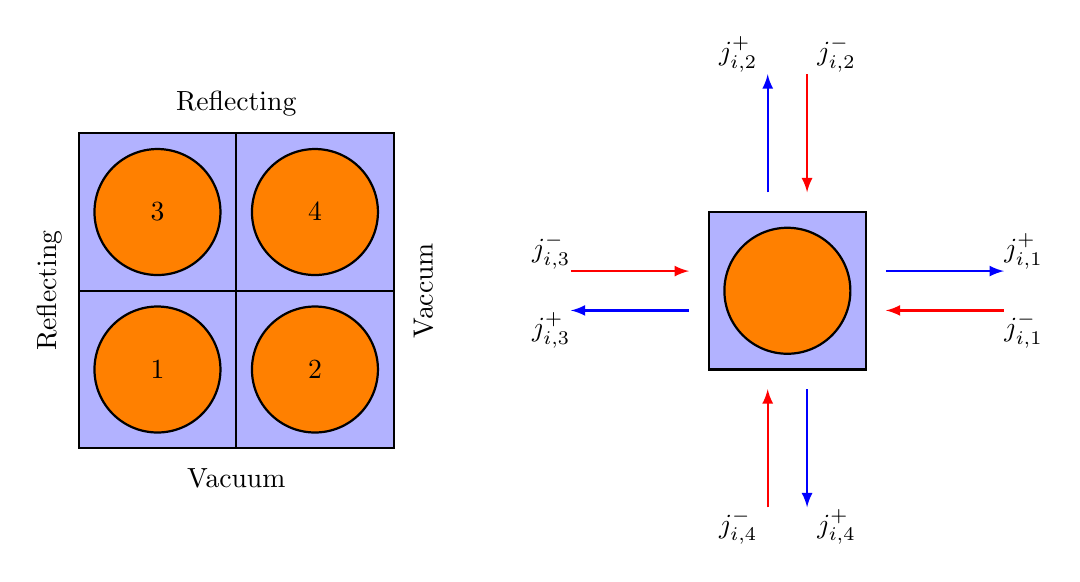
\begin{tikzpicture}

\filldraw[thick,fill=blue!30] (-1,0) -- (3,0) -- (3,4) -- (-1,4) -- cycle;
%\node at (0,-0.5*\h*\a+0.25) {$L$};

\draw[thick] (-1,2) -- (3,2);
\draw[thick] ( 1,0) -- (1,4);

\foreach \i in {-1,1} {
  \foreach \j in {0,2} {
    \filldraw[thick,fill=orange] ({\i+1},{\j+1}) circle (0.8cm);
  }
}

\node at (0,1) {1};
\node at (2,1) {2};
\node at (0,3) {3};
\node at (2,3) {4};

\node[rotate=90] at ( 3.375,2) {Vaccum};
\node[rotate=90] at (-1.375,2) {Reflecting};

\node at (1, 4.375) {Reflecting};
\node at (1,-0.375) {Vacuum};


\filldraw[thick,fill=blue!30] (7,1) -- (9,1) -- (9,3) -- (7,3) -- cycle; 
\filldraw[thick,fill=orange]  (8,2) circle (0.8cm); 

\draw[-latex,thick,blue] ( 9.25, 2.25) -- (10.75, 2.25);
\draw[-latex,thick,blue] ( 7.75, 3.25) -- ( 7.75, 4.75);
\draw[-latex,thick,blue] ( 6.75, 1.75) -- ( 5.25, 1.75);
\draw[-latex,thick,blue] ( 8.25, 0.75) -- ( 8.25,-0.75);


\draw[-latex,thick,red]  (10.75, 1.75) -- ( 9.25, 1.75);
\draw[-latex,thick,red]  ( 8.25, 4.75) -- ( 8.25, 3.25);
\draw[-latex,thick,red]  ( 5.25, 2.25) -- ( 6.75, 2.25);
\draw[-latex,thick,red]  ( 7.75,-0.75) -- ( 7.75, 0.75);

\node at (11,2.5) {$j^+_{i,1}$};
\node at (11,1.5) {$j^-_{i,1}$};

\node at (7.375,5) {$j^+_{i,2}$};
\node at (8.625,5) {$j^-_{i,2}$};

\node at (5,1.5)   {$j^+_{i,3}$};
\node at (5,2.5)   {$j^-_{i,3}$};

\node at (8.625,-1) {$j^+_{i,4}$};
\node at (7.375,-1) {$j^-_{i,4}$};

\end{tikzpicture}

\caption{Example illustrating layout of connectivity matrix.}
\label{Fig:transport_connectivityExample}
\end{center}
\end{figure}

We provide an example illustrated in Fig.~\ref{Fig:transport_connectivityExample} to show the connectivity matrix. In this example, we have a simple 2$\times$2 array of four different cells with potentially different material properties. The top and left boundary conditions are reflecting and the bottom and right are vacuum. We index the four edges/faces starting at the right element and going counter-clockwise. The number of rows and columns is the number of cells (four) times the number of edges per cell (four) for a total of 16, giving a 16$\times$16 matrix. We order the matrix such that each unit cell forms a 4$\times$4 block (corresponding to the number of faces/edges) in the bigger matrix. The rows and columns within each block represent the contained faces/edges in the prescribed ordering.

The connectivity matrix in this example is then
\begin{align}
  \mathbf{M} = \left[ \begin{array}{c c c c|c c c c|c c c c|c c c c}
  0 & 0 & 0 & 0 &		0 & 0 & 1 & 0 &			0 & 0 & 0 & 0 &			0 & 0 & 0 & 0 \\
  0 & 0 & 0 & 0 &		0 & 0 & 0 & 0 &			0 & 0 & 0 & 1 &			0 & 0 & 0 & 0 \\  
  0 & 0 & 1 & 0 &		0 & 0 & 0 & 0 &			0 & 0 & 0 & 0 &			0 & 0 & 0 & 0 \\
  0 & 0 & 0 & 0 &		0 & 0 & 0 & 0 &			0 & 0 & 0 & 0 &			0 & 0 & 0 & 0 \\ \hline
%
  0 & 0 & 0 & 0 &		0 & 0 & 0 & 0 &			0 & 0 & 0 & 0 & 		0 & 0 & 0 & 0 \\
  0 & 0 & 0 & 0 &		0 & 0 & 0 & 0 &			0 & 0 & 0 & 0 & 		0 & 0 & 0 & 1 \\
  1 & 0 & 0 & 0 &		0 & 0 & 0 & 0 &			0 & 0 & 0 & 0 & 		0 & 0 & 0 & 0 \\
  0 & 0 & 0 & 0 &		0 & 0 & 0 & 0 &			0 & 0 & 0 & 0 & 		0 & 0 & 0 & 0 \\ \hline
%
  0 & 0 & 0 & 0 &		0 & 0 & 0 & 0 &			0 & 0 & 0 & 0 & 		0 & 0 & 1 & 0 \\
  0 & 0 & 0 & 0 &		0 & 0 & 0 & 0 &			0 & 1 & 0 & 0 & 		0 & 0 & 0 & 0 \\
  0 & 0 & 0 & 0 &		0 & 0 & 0 & 0 &			0 & 0 & 1 & 0 & 		0 & 0 & 0 & 0 \\
  0 & 1 & 0 & 0 &		0 & 0 & 0 & 0 &			0 & 0 & 0 & 0 & 		0 & 0 & 0 & 0 \\ \hline
%  
  0 & 0 & 0 & 0 &		0 & 0 & 0 & 0 &			0 & 0 & 0 & 0 & 		0 & 0 & 0 & 0 \\
  0 & 0 & 0 & 0 &		0 & 0 & 0 & 0 &			0 & 0 & 0 & 0 & 		0 & 1 & 0 & 0 \\
  0 & 0 & 0 & 0 &		0 & 0 & 0 & 0 &			1 & 0 & 0 & 0 & 		0 & 0 & 0 & 0 \\
  0 & 0 & 0 & 0 &		0 & 1 & 0 & 0 &			0 & 0 & 0 & 0 & 		0 & 0 & 0 & 0 \\ \end{array} \right] .
\end{align}

Returning to Eq.~\eqref{Eq:transport_transmissionProbabilityMethod_relateCurrents} and inserting the connectivity matrix, we can solve for the outward partial current vector in terms of the currents because of the internal source:
\begin{align}
  \mathbf{j}^+ = \left( \mathbf{I} - \mathbf{R} \mathbf{M} \right)^{-1} \mathbf{j}^s .
\end{align}
Multiplying by the connectivity matrix we can then get the inward partial currents as
\begin{align} \label{Eq:transport_inwardPartialCurrent_responseMatrix_finalResult}
  \mathbf{j}^- = \mathbf{M} \left( \mathbf{I} - \mathbf{R} \mathbf{M} \right)^{-1} \mathbf{j}^s .
\end{align}

Given the inward partial currents, we can now use Eq.~\eqref{Eq:transport_transmissionProbability_cellCollisionRate} to solve for the cell collision rate---or equivalently the group scalar flux---in each region:
\begin{align} \label{Eq:transport_collisionRates_responseMatrix_finalResult}
  f_i = \Sigma_{t,i} A_i \phi_i 
  = \frac{ \Sigma_{t,i} }{ \Sigma_{t,i} - \Sigma_{s,i} P_{ii} } \left[ P_{ii} S_i A_i + \displaystyle\sum_{j \in i} P_{i,b_j} j^-_{i,b_j} \right] .
\end{align}
Here the sum is over all faces of region $i$.




\subsection{Homogenization}

We have equations calculating the inward partial currents and the resulting group scalar fluxes, but they need the collision and boundary crossing probabilities, which can be obtained from Eqs.~\eqref{Eq:transport_collisionProbabilities2D_rayTracing}. Here we only need the case of the self collision probability since we define each region to contain a single region for which a spatially flat source is a suitable approximation. 

The difference from what we did in the previous section on the collision probability method is that we do cylindricize the unit cell, but rather we (usually) homogenize to simplify the internal structure of each unit cell such that the boundaries are rectangular. The simplest case of this is to completely homogenize the cell such that it contains a single material. We make both simplifications of rectangular regions containing a single material here.

The first step in this process is to homogenize each typical unit cell using the fluxes we obtained from the collision probability method. Doing this, however, will not necessarily preserve reaction rates, so we need to use an iterative scheme to find equivalent cross section. The first guess for the homogeneous group cross sections is done using flux-volume weighting:
\begin{align}
  \overline{\Sigma}_{x,I,g}^{(0)} = \dfrac{ \displaystyle\sum_{i \in I} \Sigma_{x,i,g} \phi_{i,g} A_i }{  \displaystyle\sum_{i \in I} \phi_{i,g} A_i } .
\end{align}
Here we let $i$ be the index of the unit cell spatial region corresponding to the homogenized region $I$ in some lattice or array. We may encounter a case where there is no representative flux spectrum available, e.g., in some gap outside the assembly. In this case, we either pick the closest one we have, or we do simple volume homogenization.

As mentioned, these do not preserve the reaction rates within the heterogeneous unit cell. The collision rate is given by
\begin{align}
  R_g = \sum_i \Sigma_{t,i,g} A_i \phi_{i,g} .
\end{align}
Correcting for the heterogeneous collision rate involves performing another collision probability calculation using the homogenized cross section $\overline{\Sigma}_{x,I,g}^{(0)}$ distributed throughout the cylindricized unit cell volume instead of the actual heterogenous materials. From this calculation, we obtain group fluxes $\phi^{(0)}_{i,g}$ that we use to obtain collision rates
\begin{align}
  R_g^{(n)} = \sum_i \overline{\Sigma}_{x,I,g}^{(n)} A_i \phi_{i,g}^{(n)} .
\end{align}
The corrected cross section is then the ratio of the reaction rates times the previous cross section. Writing this for generic iteration index $n$, we have
\begin{align}
   \overline{\Sigma}_{x,I,g}^{(n+1)} = \frac{ R_g }{ R_g^{(n)} } \overline{\Sigma}_{x,I,g}^{(n)} .
\end{align}
We continue this iteration until the homogenized cross sections converge within some tolerance.

For standard fuel pins, the correction for homogenization is typically close to one for most of the energy groups. The correction factors are particularly far from one for thermal groups in cases with strong thermal absorbers such as fuel pins with burnable absorbers or control elements. Performing this correction yields more representative spectra for the energy condensation procedure.




\subsection{Ray-Tracing Calculation}

\begin{figure}[tb!]
\begin{center}

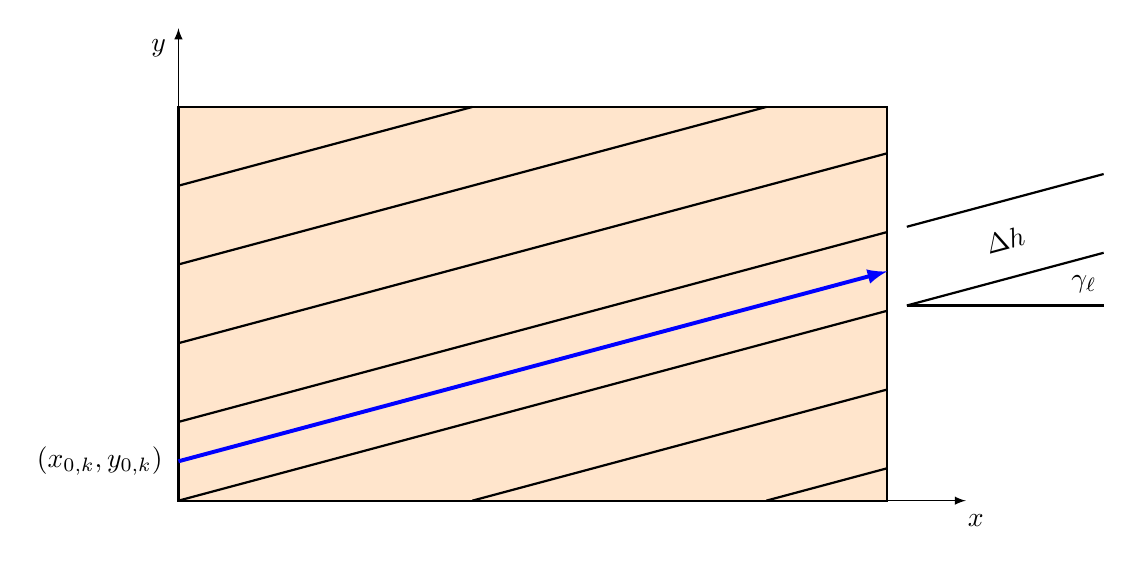
\begin{tikzpicture}

\filldraw[thick,fill=orange!20] (0,0) -- (9,0) -- (9,5) -- (0,5) -- cycle;

\draw[-latex] (0,0) -- (10,0);
\draw[-latex] (0,0) -- (0,6);
\node at (10.125,-0.25) {$x$};
\node at (-0.25,5.75)  {$y$};


\foreach \j in {-2,-1,0,1,2,3,4} {
%  \draw[thick] ( {max(0, -0.25/tan(15) - \j/tan(15)) } , {max( 0, 0.25 + \j)} ) -- ( {min( 9, 4.75/tan(15) - \j/tan(15) ) }  , {min( 5, 0.25 + \j + 9*tan(15) )} );
  \draw[thick] ( {max(0,  - \j/tan(15)) } , {max( 0, \j)} ) -- ( {min( 9, 5/tan(15) - \j/tan(15) ) }  , {min( 5, \j + 9*tan(15) )} );
}

\draw[thick] (9.25,{ 0 + 9.25*tan(15) }) -- (11.75,{ 0 + 11.75*tan(15) });
\draw[thick] (9.25,{ 1 + 9.25*tan(15) }) -- (11.75,{ 1 + 11.75*tan(15) });
\draw[thick] (9.25,{ 0 + 9.25*tan(15) }) -- (11.75,{ 0 +  9.25*tan(15) });

%\draw[thick] (9.25,{ 0.25 + 9.25*tan(15) }) -- (11.75,{ 0.25 + 11.75*tan(15) });
%\draw[thick] (9.25,{ 1.25 + 9.25*tan(15) }) -- (11.75,{ 1.25 + 11.75*tan(15) });
%\draw[thick] (9.25,{ 0.25 + 9.25*tan(15) }) -- (11.75,{ 0.25 +  9.25*tan(15) });

\draw[-latex,line width=0.5mm,blue] (0,0.5) -- (9,{ 0.5 + 9*tan(15) });
\node at (-1,0.5) {$(x_{0,k},y_{0,k})$};

\node[rotate=15] at (10.5,{ 0.5 +  10.5*tan(15) }) {$\Delta h$};
\node at (11.5,2.75) {$\gamma_\ell$};

%\foreach \j in {-1,0,1,2,3,4} {
%  \draw[thick] ( { max( -0.25/tan(15) - \j/tan(15), 0 ) } , {max(\j + 0.25,0} ) -- ( { min( 5.5/tan(15) - \j/tan(15), 9 ) },  {min(\j + 0.25 + 5*tan(15),5)} );
%}



\end{tikzpicture}

\caption{Depiction of ray tracing through a rectangular region.}
\label{Fig:transport_rayTracingRectangularRegion}
\end{center}
\end{figure}

The homogenization procedure discussed in the previous section simplifies the ray tracing algorithm because each ray only requires a single segment because the material properties are uniform. On the other hand, we do not have radial symmetry, so we have to actually carry out the azimuthal integration. This is done by evaluating Eqs.~\eqref{Eq:transport_collisionProbabilities2D_rayTracing} numerically using a series of parallel rays for a set of azimuthal inclinations~$\gamma_\ell$. For simplicity, we let there be an equal ray spacing $\Delta h$ that is independent of $\gamma_\ell$. An example of typical rays going through a rectangular region is depicted in Fig.~\ref{Fig:transport_rayTracingRectangularRegion}.

Suppose there are $L$ azimuthal inclinations that are equally spaced from $(0,\pi)$. This means we have the azimuthal spacing and angles of
\begin{align}
  \Delta \gamma = \frac{\pi}{L}, \quad \gamma_\ell = \left( \frac{ 2\ell - 1 }{2} \right) \Delta \gamma , \quad \ell = 1, \ldots, L .
\end{align}
Note that this intentionally excludes rays that are orthogonal to the $x$ and $y$ axes, which avoids having to treat the special case where a ray could be collinear with an edge. Because rays can be traced in either direction, we only need to perform the tracing over half of the space and the results can be multiplied by two.

To generate rays for each azimuthal inclination, we can first subdivide the geometry into a series of slices along one the principal axes, suppose the $x$ axis. We can then put rays at the midpoints of each segment. Then, for each ray $k$ having azimuthal inclination $\gamma_\ell$, we need to compute the edge that the ray enters, the location of entry $(x_{0,k},y_{0,k})$ into the region, and the segment length $s_{k,\ell}$ and the corresponding optical depth $\tau_{k,\ell}$. To illustrate, in the figure, the ray drawn enters through the left edge and exits through the right edge. If we were to cast a similar ray for the slice immediately below, then the ray would enter through the bottom edge instead while still leaving through the right edge.

Given this information can be calculated for every ray. We have an outer loop over each azimuthal inclination $\gamma_\ell$ and an inner loop over each ray $k$ the intersects with the region. Based on this, we can estimate the intensities $T$. These intensities are related to the first-flight probabilities by
\begin{subequations}
\begin{align}
  T_{i,i}   	 &= \Sigma_{t,i} A_i P_{i,i} , \\
  T_{b_j,i} 	 &= \Sigma_{t,i} A_i P_{b_j,i} , \\
  T_{i,b_j}      &= \frac{L_j}{4} P_{i,b_j}, \\
  T_{b_{j'},b_j} &= \frac{L_j}{4} P_{b_{j'},b_j} . 
\end{align}
\end{subequations}
The second index denotes the starting point and the first index denotes the end point where the $b$ subscript is used to denote entering at edges. The factor of four arises on the intensities starting at an edge because we assume an isotropic angular flux at the boundaries.

Using Eqs.~\eqref{Eq:transport_collisionProbabilities2D_rayTracing}, we obtain the intensities as
\begin{subequations}
\begin{align}
  T_{i,i} &= \Sigma_{t,i} A_i - \frac{ 2 \Delta\gamma \Delta h }{ \pi } \sum_\ell \sum_k \left[ \frac{\pi}{4} - \kin_3( \tau_{k,\ell} ) \right] , \\
  T_{b_{j},i} &= \frac{ 2 \Delta\gamma \Delta h }{ \pi } \sum_\ell \sum_{ k \in b_j } \left[ \frac{\pi}{4} - \kin_3( \tau_{k,\ell} ) \right] , \\
  T_{b_{j},b_{j'}} &= \frac{ 2 \Delta\gamma \Delta h }{ \pi } \sum_\ell \sum_{ k \in b_{j',j} } \kin_3( \tau_{k,\ell} ) ,
\end{align}
and the remaining intensity is
\begin{align}
  T_{i,b_{j}} &= T_{b_{j},i} ,
\end{align}
\end{subequations}
by way of the reciprocity relationship in Eq.~\eqref{Eq:transport_reciprocityRelation_region_segment}.

Once we have the collision intensities for each region, we can compute the corresponding collision probabilities for given energy group. These can then be used to calculate the source-driven current $\mathbf{j}^s$ vector and the response matrix $\mathbf{R}$. Then, we can solve for the inward partial currents using Eq.~\eqref{Eq:transport_inwardPartialCurrent_responseMatrix_finalResult}. Finally, we can use those partial currents along with the probabilities obtain the group fluxes within each homogenized region using Eq.~\eqref{Eq:transport_collisionRates_responseMatrix_finalResult}.

Once the fluxes for the energy group are known, we then compute the inscattering source for the next energy group and repeat the process for each group. This is discussed in greater detail next.

\subsection{Energy-Group Coupling and Rebalance}

As with the collision probability calculations, the response matrix calculations must be coupled between energy groups. The process is much that same except now we have an extra outer iteration for the fission source. In other words, we assume a fixed (now region-dependent) fission source and then solve for the group fluxes through the slowing down range. We then iterate over the group fluxes as before, but we wait to perform a rebalance until after the completing the calculations for the outer iteration. 

In the outer iteration, we use the converged group fluxes to compute a new fission source and estimate the eigenvalue $k$ of the array. Before proceeding to check convergence to determine whether another outer iteration is needed, we perform a rebalance to ensure neutron conservation.

We do not repeat the steps for the inner iteration here, as this is covered in detail in Sec.~\ref{Sec:transport_collsionProbability_energyGroupCoupling}. For outer iteration $n$, the internal source term for group $g$ within homogenized region $I$ is 
\begin{align}
  S_{I,g} = 
  \sum_{\substack{g' = 1\\ g' \ne g}}^G \Sigma_{s,I,g' \rightarrow g} \phi_{I,g'} 
  + \frac{1}{k^{(n)}} \chi_{g} \sum_{g'=1}^G \nu\Sigma_{f,I,g'} \phi_{I,g'}^{(n)} .
\end{align}
Per the discussion in the other section, the inscatter source is updated within the inner iteration and hence it does not obtain an iteration index $n$, i.e., only terms fixed within and updated after the outer iterations have an iteration superscript here, namely the flux used to compute the fission source and the eigenvalue $k$.

After completion of the outer iteration, we perform a fundamental mode rebalance on the flux we just obtained, $\phi^{(n+1)}$. We first compute the volume-averaged cross sections over the entire problem geometry as before,
\begin{align}
  \overline{\Sigma}_{x,g} = \dfrac{ \displaystyle\sum_I \Sigma_{x,I,g} \phi_{I,g}^{(n+1)} A_I }{ \displaystyle\sum_I \phi_{I,g}^{(n+1)} A_I } ,
\end{align}
but this time summed over the homogenized lattice cells. Next, we compute the volume-averaged group fluxes by solving the neutron balance equation,
\begin{align}
  \overline{\Sigma}_{R,g} \overline{\phi}_g = \sum_{\substack{g' = 1\\ g' \ne g}}^G \Sigma_{s,I,g' \rightarrow g} \overline{\phi}_{g'}  
  + \frac{\chi_{g}}{k^{(n)}}  \sum_{g'=1}^G \nu\Sigma_{f,I,g'} \overline{\phi}_{g'} .
\end{align}

Once we have the volume-averaged scalar fluxes, we then compute a new eigenvalue for the next iteration,
\begin{align}
  k^{(n+1)} =  \dfrac{ \displaystyle\sum_g \overline{ \nu \Sigma }_{f,g} \overline{\phi}_g }{ \displaystyle\sum_g \overline{ \Sigma }_{a,g} \overline{\phi}_g } .
\end{align}
We rescale the fluxes for the next iteration using
\begin{align}
  \hat{\phi}_{I,g}^{(n+1)} = \phi_{I,g}^{(n+1)} \dfrac{ \overline{\phi}_g }{ \displaystyle\sum_I \phi_{I,g}^{(n+1)} A_I } .
\end{align}
We finally check convergence of the eigenvalue and the fluxes. If they are not converged, we use $\hat{\phi}_{I,g}^{(n+1)}$ to compute the fission source in the next iteration and repeat until the flux converges.




\subsection{Condensation Scheme}

Once we have converged group fluxes on the homogenized lattice array, we then use those to condense the group cross sections from the fine group structure into a coarse group structure using the appropriate flux spectrum for each unit cell in the lattice. This leads to a much smaller number of energy groups to iterate over in a detailed transport calculations even though the number of region cross sections may be larger accounting for the spatial variation of the fluxes.

The first step in the condensation scheme is to determine the flux spectrum for each individual region within every unit cell. We base this on the detailed flux spectrum for the corresponding representative unit cell that we determined using the collision probability calculation as well as the local response matrix calculation. Taken together, the local flux spectrum is
\begin{align}
  \phi_{i,I,g} = \phi_{i,g} \dfrac{ \phi_{I,g} A_I }{ \displaystyle\sum_{i \in I} \phi_{i,g} A_i } .
\end{align}
Here again $i$ denotes the spatial index in the representative 1-D unit cell calculation and $I$ denotes the spatial index of the homogenized region in the 2-D response matrix calculation. The group flux on the left-hand side shares both spatial indices denoting it is for a particular region in specific unit cell within the 2-D lattice.

As before, $g$ is the index denoting the fine energy group $E_g \le E < E_{g-1}$. We let $h$ be the index denoting the coarse energy group $E_h \le E < E_{h-1}$, which contains several energy groups $g$. The local reaction cross section for the coarse group $h$ is then
\begin{align}
  \Sigma_{x,i,I,h} = \dfrac{ \displaystyle\sum_{h \in g} \Sigma_{x,i,g} \phi_{i,I,g} }{ \displaystyle\sum_{h \in g} \phi_{i,I,g}  } .
\end{align}
These region-wise cross sections are then used in the downstream calculations for assembly-level transport calculations, discussed in the remainder of this chapter, and the full-core diffusion calculations covered in the next chapter.






%%%%%%%%%%%%%%%%%%%%%%%%%%%%%%%%%%%%%%%%%%%%%%%%%%%%%%%%%%%%%%%%%%%%%%%%%%%%%%%%%%%%%%%%%%%%%%%%%%%%
\section{Discrete Ordinates in 1-D Slab Geometry}

In this section we begin the discussion the transport-based discrete ordinates (or segment-$N$) method that can be used to obtain spatially dependent fluxes on the assembly or few-assembly scale. Here we limit the scope to the simplest case of 1-D slab or planar geometry. In the next section we extend this to two spatial dimensions on a Cartesian grid.  The discrete ordinates method can further be extended to unstructured mesh geometry or curvilinear coordinates, but we set those outside the scope of this text.

The discrete ordinates method is very similar to the classic finite difference method used to solve a wide variety of differential equations encountered in physics, e.g., the Poisson equation for the transport of thermal energy. The idea is that the spatial domain is discretized by integrating over discrete regions and particles are restricted to traveling along discrete directions or ordinates. This permits us to write a system of coupled equations with one equation for each spatial domain and for each direction. This, in effect, is a linear algebra problem for which we have well-established solution techniques.

\subsection{Advantages and Disadvantages}

One question is why we simply the collision probability method is not adequate for the task. After all, we use a transmission-probability variant with a response matrix to analyze an assembly in the previous section. The answer to this is in the earlier sections, we are most concerned with either the fine-group spectral details at the resolution of an individual unit cell. The response matrix method serves as a way to correct the spectrum for the effect of neighboring unit cells, but does not really get the spatial details very accurately.

To review, the collision probability method has a few major shortcomings that limits its applicability beyond individual unit cells. The first is that it is largely restricted to isotropic scattering and boundary fluxes. In principle it is possible to build in higher scattering moments, but doing so largely removes the advantages of the method. Additionally, applying a transport correction to the total and within-group scattering cross section is often adequate. The second is that we have to assume the flat source approximation within each cell. Again, we can relax this assumption, but at a significant computational expense. And finally, the collision probability method requires the inversion of large and dense matrices. The size of these matrices grows rapidly with the number of spatial elements, which means the time to solution grows unfavorably as well.

So if we abandon the collision probability method, the next question is why discrete ordinates. Admittedly, the short answer is that it is not the best choice for assembly calculations given modern computing resources. The superior method for this particular application is the method of characteristics, which shares many common algorithmic features, i.e., ray tracing based, with the collision probability method. 

Discrete ordinates, on the other hand, is exceptionally versatile and largely the workhorse for general transport problems involving anisotropy, applicable to reactor analysis, shielding, radiation detection, and other applications. Whereas the method of characteristics excels in applications where there is a relatively uniform source distribution, the angular flux is not too anisotropic, and significant heterogeneity in two spatial dimensions, but not too much in the third---all features of a fuel assembly in a conventional reactor. Because discrete ordinates is so broadly applicable, we devote a section to the method.

Before delving into the method, we should also comment that there are other transport methods we could have chosen. The first of these is the spherical harmonics expansion or P$_N$ method, which can be thought of as a higher-order expansion of classic diffusion theory. This method works well in diffusive problems, but becomes either inaccurate or computationally costly when high-order anisotropy in the angular flux is present. 

Another class are schemes based on the second-order even-parity or self-adjoint angular flux formulations of the transport equation. These are attractive because they lend themselves well to traditional continuous finite element based schemes used in fields of structural mechanics or heat transfer. The disadvantage is the matrices become ill conditioned for optically thin media and become singular in voids, which cause major issues for a set of applications. 

Finally, there is the Monte Carlo method, which is gaining traction in the area of reactor analysis. The method is based on random sampling and carries minimal approximations in the physics, meaning that it is, like discrete ordinates, exceptionally versatile. Further, the lack of approximations and user input parameters leads to a significant advantage in that the learning curve to use Monte Carlo-based computational tools is much lower than the alternatives. The major drawback is that it is by far the most computationally costly method available and has been deemed the ``method of last resort''.

%This section is organized into two parts. The first covers the case of 1-D slab geometry transport methods. These are relatively straightforward and serve as a way to introduce the method without all the complexities that arise from multiple dimensions or curvilinear geometry. The second part applies the discrete ordinates method to the case of 2-D rectangular grids. The discrete ordinates method can further be extended to unstructured mesh geometry or curvilinear coordinates, but we set those outside the scope of this text.

%\subsection{Neutron Transport 1-D Discrete Ordinates Method}
%
%To begin this, we write the steady-state, 1-D neutron transport equation in slab geometry as
%\begin{align}
%  \mu \dho{}{x} \psi(x,\mu) + \Sigma_t(x) \psi(x,\mu) = q(x,\mu) ,
%\end{align}
%where, for compactness, we lumped scattering, fission, and internal sources into the right-hand side source $q(x,\mu)$. We have two independent variables, the spatial coordinate $x$ and the direction cosine $\mu$ with respect to the $x$-axis. Both of these need to be discretized in some manner.

\subsection{Spatial Discretization}

\begin{figure}[tb!]
\begin{center}
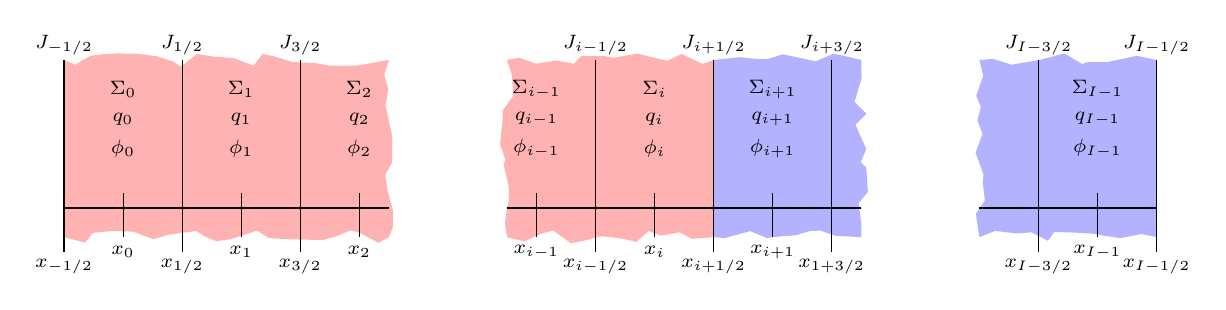
\begin{tikzpicture}[scale=0.75] \scriptsize
% left side boundary section
\fill[red!30, decoration={random steps,segment length=0.2cm}] (0,-0.5) decorate{-- (5.5,-0.5)} decorate{-- (5.5,2.5)} decorate{-- (0,2.5)} -- cycle;
\draw[thick] (0,0) -- (5.5,0);
\draw (0,-0.75) -- (0,2.5);
\draw (1,-0.5)  -- (1,0.25);
\draw (2,-0.75) -- (2,2.5);
\draw (3,-0.5)  -- (3,0.25);
\draw (4,-0.75) -- (4,2.5);
\draw (5,-0.5)  -- (5,0.25);
\node at (0,-1) 	{$x_{-1/2}$};
\node at (1,-0.75) 	{$x_0$};
\node at (2,-1) 	{$x_{1/2}$};
\node at (3,-0.75) 	{$x_1$};
\node at (4,-1) 	{$x_{3/2}$};
\node at (5,-0.75) 	{$x_2$};
\node at (0,2.75) {$J_{-1/2}$}; \node at (2,2.75) {$J_{1/2}$}; \node at (4,2.75) {$J_{3/2}$};
\node at (1,2)   {$\Sigma_0$}; \node at (1,1.5)   {$q_0$}; 	\node at (1,1)   {$\phi_0$};
\node at (3,2)   {$\Sigma_1$}; \node at (3,1.5)   {$q_1$}; 	\node at (3,1)   {$\phi_1$};
\node at (5,2)   {$\Sigma_2$}; \node at (5,1.5)   {$q_2$}; 	\node at (5,1)   {$\phi_2$};

% interior section
\fill[red!30,  decoration={random steps,segment length=0.2cm}] (7.5,-0.5) decorate{-- (11,-0.5)} -- (11,2.5) decorate{-- (7.5,2.5)} decorate{-- cycle};
\fill[blue!30, decoration={random steps,segment length=0.2cm}] (11,-0.5)  decorate{-- (13.5,-0.5)} decorate{-- (13.5,2.5)} decorate{-- (11,2.5)} -- cycle;
\draw[thick] (7.5,0) -- (13.5,0);
\draw (8, -0.5)   -- (8, 0.25);
\draw (9, -0.75)  -- (9, 2.5);
\draw (10,-0.5)   -- (10,0.25);
\draw (11,-0.75)  -- (11,2.5);
\draw (12,-0.5)   -- (12,0.25);
\draw (13,-0.75)  -- (13,2.5);
%\draw (14,-0.5)   -- (14,0.25);
\node at (8,-0.75) 	{$x_{i-1}$};
\node at (9,-1) 	{$x_{i-1/2}$};
\node at (10,-0.75) {$x_{i}$};
\node at (11,-1) 	{$x_{i+1/2}$};
\node at (12,-0.75) {$x_{i+1}$};
\node at (13,-1) 	{$x_{1+3/2}$};
%\node at (14,-0.75) {$x_{i+2}$};
\node at (9,2.75) {$J_{i-1/2}$}; \node at (11,2.75) {$J_{i+1/2}$}; \node at (13,2.75) {$J_{i+3/2}$};
\node at (8, 2)   {$\Sigma_{i-1}$}; 	\node at (8, 1.5) {$q_{i-1}$}; 	\node at (8, 1)   {$\phi_{i-1}$};
\node at (10,2)   {$\Sigma_{i}$}; 		\node at (10,1.5) {$q_{i}$}; 	\node at (10,1)   {$\phi_{i}$};
\node at (12,2)   {$\Sigma_{i+1}$}; 	\node at (12,1.5) {$q_{i+1}$}; 	\node at (12,1)   {$\phi_{i+1}$};
%\node at (14,2)   {$\Sigma_{i+2}$}; 	\node at (14,1.5) {$q_{i+2}$}; 	\node at (14,1)   {$\phi_{i+2}$};

% interior section
\fill[blue!30,  decoration={random steps,segment length=0.2cm}] (15.5,-0.5) decorate{-- (18.5,-0.5)} -- (18.5,2.5) decorate{-- (15.5,2.5)} decorate{-- cycle};
\draw[thick] (15.5,0) -- (18.5,0);
\draw (18.5, -0.75)   -- (18.5, 2.5);
\draw (17.5, -0.5)  -- (17.5, 0.25);
\draw (16.5, -0.75)  -- (16.5, 2.5);
\node at (16.5,-1) 	{$x_{I-3/2}$};
\node at (17.5,-0.75) {$x_{I-1}$};
\node at (18.5,-1) 	{$x_{I-1/2}$};
\node at (16.5,2.75) {$J_{I-3/2}$}; \node at (18.5,2.75) {$J_{I-1/2}$};
\node at (17.5, 2)   {$\Sigma_{I-1}$}; 	\node at (17.5, 1.5) {$q_{I-1}$}; 	\node at (17.5, 1)   {$\phi_{I-1}$};

\end{tikzpicture}
\caption{Grid or stencil for the cell-centered finite differencing scheme for the numerical solutions of neutron transport and diffusion.}
\label{Fig:neutronics_finiteDifferenceStencil}
\end{center}
\end{figure}

To begin we return the steady-state, 1-D neutron transport equation in slab geometry for a single energy group:
\begin{align}
  \mu \dho{}{x} \psi(x,\mu) + \Sigma_t(x) \psi(x,\mu) = q(x,\mu) ,
\end{align}
This angular flux has two dimensions: the spatial $x$ coordinate in a 1-D slab (where the geometry, sources, and boundary conditions are infinite and uniform in the $y$ and $z$ directions) and the angular variable $\mu$, which is the cosine of the angle of neutron flight with respect to the $x$ axis. (Recall the symmetry of the problem means the angular flux is uniform in the azimuthal directional variable.) To solve this problem, we need to apply a discretization in both of these variables.

First, we introduce \emph{cell-centered} spatial discretization, which is depicted in Fig.~\ref{Fig:neutronics_finiteDifferenceStencil}. The rationale of this choice is it allows us to strictly enforce particle balance within each zone where outgoing currents $J$ are given on the edges and reaction rates, by way of the scalar flux $\phi$, are defined at the center. The concept of particle balance states simply that the rate particles are produced from the source plus the rate particles enter must be balanced by the rate particles are absorbed plus the rate they leave. 

This sounds rather obvious, but just because the differential equation of neutron transport naturally preserves particle balance by virtue of how it was derived, the process of mapping that differential equationsonto a spatial discretization, which converts a calculus problem into algebra one, may or may not preserve the balance of particles depending on how this is done. Enforcing particle balance (or analogously conservation of mass, momentum, and energy if we were solving a thermal fluids problem) has a cost, and that is a more complicated numerical scheme.

The cell-centered spatial discretization breaks the problem into $I$ spatial regions indexed from $i = 0, 1, \ldots, I-1$ (indexing from zero follows the convention from the C programming language that most modern languages use) each having a width $\Delta_i = x_{i+1} - x_i$. The point $x_i$ is the center of the $i$th spatial zone. This implies that $x_{-1/2} = 0$ is the left edge of the slab and $x_{I-1/2} = a$ is the right edge. Material properties (e.g., cross sections) and sources are taken to be within each spatial zone. Ideally, we choose the spatial discretization to line up with the geometric regions of the problem. If we cannot do this, or do not wish to for some reason, then we need to find some average value of the material properties.




\subsection{Angular Discretization with Gauss-Legendre Quadrature}

We also need to discretize the direction or angular variable $\mu$. As the name of the discrete ordinates method implies, we pick a set of discrete directions $\mu_n$ that the neutrons travel along. We have a large amount of flexibility to pick the angular discretization, but in 1-D planar geometry there is one choice that is usually superior to anything else, which is picking the $\mu_n$ to be along the Gauss-Legendre quadrature integration points. Why this is is because the right-hand side $q(x,\mu)$ includes the scattering and fission sources that contain integrals over the angular fluxes. It is therefore beneficial to pick a set of directions that maximize the accuracy of numerically calculating these integrals with the fewest number of points.

For those readers not familiar, with the Gauss-Legendre quadrature set, we do a quick summary. In general, we can write a quadrature rule for numerical integration from the domain of $[-1,1]$ as
\begin{align}
  \int_{-1}^1 f(\mu) d\mu \approx \sum_{n=1}^N w_n f(\mu_n) .
\end{align}
We have quite a bit of freedom to choose the points or abscissa $\mu_n$ and the associated weights $w_n$. One common constraint is to choose the weights such that it correctly integrates the special case of $f(\mu_n) = 1$, a constant. This requires that the sum of the weights add to two:
\begin{align}
  \sum_{n=1}^N w_n = 2.
\end{align}

There exists a special set of $N$ points and weights capable of \emph{exactly} integrating polynomials up an order $2N - 1$, which makes for a very attractive choice. These special points $\mu_n$ are the roots of the $N$th-order Legendre polynomial $P_N(\mu)$ for $n = 0,\ldots,N-1$. The weights can be computed from
\begin{align}
  w_n = \frac{ 2 }{ ( 1 - \mu_n^2 ) \left[ P_N'(\mu_n) \right]^2 } .
\end{align}
So if we use just four of these special points and weights, we can (almost miraculously) integrate up to a seventh-order polynomial exactly. (One might say integrating polynomials is easy, and they would not be wrong; however, the formulas for the integrals can get quite cumbersome and it is usually the case that just using these points and weights is much quicker from both an implementation and an execution standpoint.) 

In practice, the points $\mu_n$ and weights $w_n$ are pre-calculated and put into lookup tables. One nice property is that the points are always symmetric across the zero, so if $\mu_n$ is a point, then so is $-\mu_n$. Furthermore, the weights for both of these are identical. Because of this, we often only need to store half of the information and can just reuse the information for the other half. We often times colloquially refer to these as the $S_N$ Gauss-Legendre set. The case for $N = 16$ is given to high precision in Table~\ref{Table:neutronics_S16GaussLegendreQuadratureWeightsAbscissa}, which is adequate for many applications. 

Note that we usually choose $N$ to be even. The odd-ordered Gauss-Legendre quadrature set includes $\mu_{n-1} = 0$, which creates a potential ``divide by zero'' scenario that would need to be handled as a special case. To avoid having to check for and address this scenario, the simple and agreed-upon solution is just to demand even-ordered quadrature sets.

\begin{table}[tb!]
\caption{$S_{16}$ Gauss-Legendre Quadrature Weights and Abscissa}
\begin{center}
\begin{tabular}{|c|c|c|} \hline
$n$	& $w_n$					& $\mu_n$				\\ \hline
0	& 0.1894506104550685	& 0.0950125098376374	\\
1	& 0.1826034150449236	& 0.2816035507792589	\\
2	& 0.1691565193950025	& 0.4580167776572274	\\
3	& 0.1495959888165767	& 0.6178762444026438	\\
4	& 0.1246289712555339	& 0.7554044083550030	\\
5	& 0.0951585116824928	& 0.8656312023878318	\\
6	& 0.0622535239386479	& 0.9445750230732326	\\
7	& 0.0271524594117541	& 0.9894009349916499	\\ \hline
\end{tabular}
\end{center}
\label{Table:neutronics_S16GaussLegendreQuadratureWeightsAbscissa}
\end{table}%





\subsection{1-D Discrete Ordinates Transport Equation}

To proceed we now write the one-speed transport equation for neutrons moving along a single direction $\mu_n$. This is
\begin{align}
  \mu_n \dho{}{x} \psi(x,\mu_n) + \Sigma_t(x) \psi(x,\mu_n) = q(x,\mu_n) . \label{Eq:neutronics_discreteOrdinates_oneSpeedSingleOrdinateTransportEquation}
\end{align}
The right-hand source $q$ contains contributions from scattering, fission, and internal sources:
\begin{align}
  q(x,\mu_n) = \sum_{\ell=0}^L \left( \frac{2\ell+1}{2} \right) P_\ell(\mu_n) \Sigma_{s\ell}(x) \phi_\ell(x) + Q(x,\mu_n) . \label{Eq:neutronics_discreteOrdinates_oneSpeedRightHandSideSource}
\end{align}
Here $\phi_\ell(x)$ is the $\ell$th Legendre moment of the angular flux, which is approximated by
\begin{subequations}
\begin{align}
  \phi_\ell(x) = \int_{-1}^1 P_\ell(\mu) \psi(x,\mu) d\mu \approx \sum_{n=0}^{N-1} w_n P_\ell(\mu_n) \psi(x,\mu_n) ,
\end{align}
and $\phi(x)$ without the subscript is the standard scalar flux,
\begin{align}
  \phi(x) = \phi_0(x) = \int_{-1}^1 \psi(x,\mu) d\mu \approx \sum_{n=0}^{N-1} w_n \psi(x,\mu_n) .
\end{align}
\end{subequations}
Note that we truncated the sum over Legendre moments in Eq.~\eqref{Eq:neutronics_discreteOrdinates_oneSpeedRightHandSideSource} to order $L$. This is obviously necessary otherwise we would be stuck with having to compute an infinite number of Legendre moments, which would literally take forever. Usually the choice of truncation $L$ is dictated by the expansion order of the nuclear data cross section set. The higher the order, the higher the accuracy, but there is the inherent tradeoff between accuracy and cost in terms of computational time and memory storage requirements.

We then integrate the transport equation in Eq.~\eqref{Eq:neutronics_discreteOrdinates_oneSpeedSingleOrdinateTransportEquation} over a spatial zone or cell. Assuming constant material properties within each cell, we obtain
\begin{align}
  &\int_{x_{i-1/2}}^{x_{i+1/2}} \mu_n \dho{}{x} \psi(x,\mu_n) + \Sigma_t(x_i) \psi(x,\mu_n) dx = \int_{x_{i-1/2}}^{x_{i+1/2}}  q(x,\mu_n) dx, \nonumber \\
 &\mu_n \left[ \psi(x_{i+1/2},\mu_n) - \psi(x_{i-1/2},\mu_n) \right] + \Sigma_{t,i}  \int_{x_{i-1/2}}^{x_{i+1/2}} \psi(x,\mu_n) dx = \int_{x_{i-1/2}}^{x_{i+1/2}}  q(x,\mu_n) dx. \nonumber
\end{align}
Here we let $\Sigma_t(x_i) = \Sigma_{t,i}$. To handle the integrals, we define the cell-averaged quantities
\begin{subequations}
\begin{align}
  \psi_{i,n} 	&= \frac{1}{\Delta_i} \int_{x_{i-1/2}}^{x_{i+1/2}} \psi(x,\mu_n) dx , \\
  q_{i,n} 		&= \frac{1}{\Delta_i} \int_{x_{i-1/2}}^{x_{i+1/2}} q(x,\mu_n) dx .
\end{align}
Substituting in the definition of $q$ into the spatial integral, we see we need to also define the cell-averaged angular flux moments as
\begin{align}
  \phi_{\ell,i} &= \frac{1}{\Delta_i} \int_{x_{i-1/2}}^{x_{i+1/2}} \phi_\ell(x) dx .
\end{align}
We then note that the first term is the net flow rate for particles moving along a direction $\mu_n$. We define
\begin{align}
  J_{i+1/2,n} &= \mu_n \psi_{i+1/2,n} = \mu_n \psi(x_{i+1/2},\mu_n), \\
  J_{i-1/2,n} &= \mu_n \psi_{i-1/2,n} = \mu_n \psi(x_{i-1/2},\mu_n).
\end{align}
\end{subequations}
Given these definitions, we can then write our balance relationship for particles traveling along direction $\mu_n$ as
\begin{align}
  J_{i+1/2,n} - J_{i-1/2,n} + \Sigma_{t,i} \Delta_i \psi_{i,n} = q_{i,n} \Delta_i . \label{Eq:neutronics_discreteOrdinatesBalanceForm}
\end{align}

Before proceeding to the solution algorithm, we note that $q$ depends on the angular flux $\psi(x,\mu)$ at all $\mu_n$. One might think that one needs to store all values of $\psi(x,\mu_n)$ at all spatial grid points. It turns out this is needlessly wasteful (and impractical in 3-D calculations), and unless the angular fluxes are specifically needed, we often just keep a running sum of the Legendre moments $\phi_\ell$ at each location for elements we are not currently computing.

If we were to write out each equation for each spatial cell $i$ and ordinate $n$, we would find that we have more equations than unknowns. We therefore need to impose additional relationships to provide a mathematical closure to the equations. There are several options for doing this. Perhaps the most common is the \emph{diamond difference relationship} that says the cell-averaged angular flux is the average of the edge angular fluxes,
\begin{align}
  \psi_{i,n} = \frac{1}{2} \left( \psi_{i-1/2,n} + \psi_{i+1/2,n} \right) . \label{Eq:neutronics_diamondDifferenceRelationship}
\end{align}
The diamond difference relationship has good theoretical convergence properties, but also some important drawbacks. Namely, if spatial cells are too optically thick, then the algorithm can lead to non-physical \emph{negative} angular fluxes. In higher dimensions, it becomes difficult to avoid this occurrence and we often employ more sophisticated schemes such as linear discontinuous elements. While it is good to be aware of this, we are going to proceed anyway as a matter of expedience.




\subsection{Transport Sweep Algorithm}

The next task is to devise a numerical scheme for solving these equations. One option is to write down the equations for each pair of spatial cell $i$ and ordinate $n$, form a linear system and matrix, and solve the problem. In practice, this would be very large number of equations. While this would not be too large a system to tackle in 1-D, it becomes prohibitive in higher dimensions and with energy dependence, so we opt for a different, matrix-free method called a \emph{transport sweep}. The idea is that we order the equations in a way that we only need to solve for and store the necessary information to solve one equation at a time, discarding all variables that we will not need for subsequent equations.

The one complication here is that the source term $q$ depends on the unknown angular fluxes $\psi_{i,n}$ by way of the flux moments $\phi_{\ell,i}$. The typical way this is addressed is to use a technique called \emph{source iteration} where we guess the flux moments $\phi_{\ell,i}$, compute the sources $q_{i,n}$, solve for angular fluxes $\psi_{i,n}$ and update the flux moments. Assuming the system is subcritical, then this algorithm converges to a solution. (We will address the case of an eigenvalue problem for neutron diffusion. The idea is much the same for transport.)

To proceed with the transport sweep, we write Eq.~\eqref{Eq:neutronics_discreteOrdinatesBalanceForm} in terms of the edge-angular fluxes as
\begin{align}
  \mu_n \left[ \psi_{i+1/2,n} - \psi_{i-1/2,n} \right] + \Sigma_{t,i} \Delta_i \psi_{i,n} = q_{i,n} \Delta_i . \label{Eq:neutronics_discreteOrdinatesTransportEquation}
\end{align}
For now, we assume $q_{i,n}$ is known, and defer discussion of source iteration for a bit. The problem we have is that we have one equation for each cell, but unknowns for both the cell and the edges. First, we can handle the left and right edges via a prescribed boundary conditions:
\begin{subequations}
\begin{align}
  \psi_{-1/2,n}  &= \psi_{-1/2,n},  \quad \mu_n > 0, \\
  \psi_{I-1/2,n} &= \psi_{I-1/2,n}, \quad \mu_n < 0.  
\end{align}
\end{subequations}
(We handle the case of reflecting boundary conditions later.) This still leaves the interior edges. For this, we simply have to make an ad hoc assumption or closure that describes how the cell-average and edge angular fluxes are related, and here we apply the diamond-difference relation from Eq.~\eqref{Eq:neutronics_diamondDifferenceRelationship}.

Now we have a sufficient number of equations to solve the problem. Since for $\mu_n > 0$, we are given the information at the left boundary $\psi_{-1/2,n}^b$, we know the information on the left and can solve the equations moving from left to right in a cell-by-cell manner. Using the discrete-ordinates transport equation in Eq.~\eqref{Eq:neutronics_discreteOrdinatesTransportEquation} and the diamond difference relationship in Eq.~\eqref{Eq:neutronics_diamondDifferenceRelationship}, we arrive at the following two equations for each cell with $\mu_n > 0$:
\begin{subequations}
\begin{align}
  \psi_{i,n} &= \left( 1 + \frac{\Sigma_{t,i} \Delta_i}{ 2 | \mu_n | } \right)^{-1} \left( \psi_{i-1/2,n} + \frac{ \Delta_i q_{i,n} }{ 2 | \mu_n | } \right) , \\
  \psi_{i+1/2,n} &= 2 \psi_{i,n} - \psi_{i-1/2,n} .
\end{align}
\end{subequations}

We can then repeat this process for $\mu_n < 0$. Since we are given the right-boundary angular flux $\psi_{I-1/2,n}^b$, we solve the equations going from right to left. We obtain
\begin{subequations}
\begin{align}
  \psi_{i,n} &= \left( 1 + \frac{\Sigma_{t,i} \Delta_i}{ 2 | \mu_n | } \right)^{-1} \left( \psi_{i+1/2,n} + \frac{ \Delta_i q_{i,n} }{ 2 | \mu_n | } \right) , \\
  \psi_{i-1/2,n} &= 2 \psi_{i,n} - \psi_{i+1/2,n} .
\end{align}
\end{subequations}
Note that these results are functionally identical with the roles left- and right-edge angular fluxes swapped.

From here we can solve for all of the given angular fluxes, provided we know the right-hand side source $q_{i,n}$. As we said, in reality we do not know them because they depend on the flux moments that depend on the angular fluxes we are solving for. We address this next by bringing in source iteration.




\subsection{Negative-Flux Fixup}

One of the problems with the diamond difference relationship is that the angular fluxes can become negative as a result of spatial discretization errors. The existence of these negative fluxes adversely impacts the solution and drives instabilities in the transport sweep leading to non-convergence. 

The appearance of negative fluxes largely occurs when the cell size is too great for strongly absorbing media. For the extreme case of a 1-D pure absorber, we can derive a spatial zone size limit as
\begin{align}
  \Delta_i < \frac{ 2 | \mu_0 | }{ \Sigma_{t,i} },
\end{align}
where $| \mu_0 |$ is the minimum ordinate in the Gauss-Legendre quadrature set (not to be confused with the mean scattering cosine). The general trend here is as follows: first, the larger the total cross section, the finer the requirement on the spatial resolution. Second, the more ordinates we choose, the smaller the value of $| \mu_0 |$ we have and therefore the finer spatial resolution. Therefore, the higher we set $N$, we end up requiring a finer spatial mesh. In other words, if we refine the angular discretization variable, we also need to refine the spatial discretization in order to avoid negative fluxes and the associated numerical instabilities.

In the case of 1D, the simple solution is to simply refine the spatial mesh. In 2D or 3D, such refinement is often impractical. Therefore, we require some treatment. One possible approach is to use a different scheme that lacks the ability to have negative fluxes. This either reduces the convergence rate or requires a more complicated algorithm. 

One common compromise is to apply a set-to-zero scheme. If a negative outgoing angular flux is ever encountered, we first set that flux to zero. This alone would lead to a violation of particle balance, so we return to Eq.~\eqref{Eq:neutronics_discreteOrdinatesTransportEquation} and resolve for the cell-center angular flux. For $\mu_n > 0$ this is
\begin{align}
  \psi_{i,n} = \frac{q_{i,n}}{\Sigma_{t,i}} + \frac{\mu_n}{\Sigma_{t,i} \Delta_i } \psi_{i-1/2,n} .
\end{align}
We then use this updated cell-centered angular flux in the computation of the flux moments for that cell. We then proceed to the adjacent spatial zone with a now inward zero angular flux and continue.

This set-to-zero scheme is admittedly ad hoc and does hamper the quality of the solution somewhat. An important theoretical consideration is that the solution does not preserve the diffusive limit for scattering dominated media. While this is undesirable, it is in practice, not a major issue because negative fluxes tend to occur in media where the diffusive limit does not apply.

Another practical issue is that the set-to-zero scheme imposes a non-linear effect on the otherwise linear iteration scheme. This means that there is no guarantee the transport sweep will actually converge to an arbitrary precision. It is possible the convergence could stall out and oscillate about some usually small L$^2$ norm. For this reason, it is important to specify some maximum number of iterations in the termination criteria of the transport sweep lest the program could continue indefinitely.


\subsection{Source Iterations}

The first step of the source iteration method is we rewrite the discrete ordinates transport equation giving the angular fluxes a superscript iteration index $m$, 
\begin{align}
  \mu_n \left[ \psi_{i+1/2,n}^{(m+1)} - \psi_{i-1/2,n}^{(m+1)} \right] + \Sigma_{t,i} \Delta_i \psi_{i,n}^{(m+1)} = q_{i,n}^{(m)} \Delta_i , \label{Eq:neutronics_discreteOrdinatesTransportEquation_Iteration}
\end{align}
where the source is given in terms of the flux moments as
\begin{align}
  q_{i,n}^{(m)} = \sum_{\ell=0}^L \left( \frac{2\ell+1}{2} \right) P_\ell(\mu_n) \Sigma_{s\ell,i} \phi_{\ell,i}^{(m)}  + Q_{i,n}.
\end{align}
where the flux moments are given by
\begin{align}
  \phi_{\ell,i}^{(m)} = \sum_{n=0}^{N-1} w_n P_\ell (\mu_n) \psi_{i,n}^{(m)} 
\end{align}
with the scalar flux $\phi_i = \phi_{0,i}$. Note that the internal source $Q_{i,n}$ does not have an iteration index. In the case where the source is imposed as an inhomogeneous term, there is no need to iterate on something that is known. As with the collision probability method, the internal source contains inscattering plus fission, which is handled using separate, outer iterations.

To proceed, we make an initial guess of $\phi_{\ell,i}^{(0)}$ and compute the right-hand side source based upon that. In the absence of better information, setting them equal to zero is as good a choice as any. We then perform transport sweep to obtain $\psi_{i,n}^{(1)}$ and use these angular fluxes to obtain the flux moments $\phi_{\ell,i}^{(1)}$. We then recompute the source, perform another transport sweep, compute updated flux moments, and repeat the process. We continue this until we achieve convergence in whatever order of flux moments are needed for the output results. Often we are most interested in reaction rates, so we only need to converge the scalar fluxes. In general, however, we could converge all of them.

To measure convergence, we often use the scaled Euclidian or L$^2$ norm over all the flux moments in the problem. We compute this each iteration and stop when
\begin{align}
  \dfrac{ \left[ \displaystyle\sum_{\ell=0}^L \sum_{i=0}^{I-1} \left( \phi_{\ell,i}^{(m+1)} - \phi_{\ell,i}^{(m)} \right)^2 \right]^{1/2} }{ \left[ \displaystyle\sum_{\ell=0}^L \sum_{i=0}^{I-1} \left( \phi_{\ell,i}^{(m)} \right)^2 \right]^{1/2} } \le \epsilon,
\end{align}
where $\epsilon$ is some user-prescribed convergence tolerance for the desired level of accuracy.

Note again during transport sweeps we do not need to actually store the angular fluxes for other cells. Rather, we can accrue the updated flux moments for each spatial cell during the left and right sweeps, discarding the angular fluxes as they are no longer needed.





\subsection{Treatment of Reflecting Boundary Conditions}

In reactor analysis problems, we often solve problems with reflecting boundaries on one or often both faces to take advantage of geometric symmetry. On the left and right sides we have as the boundary conditions
\begin{subequations}
\begin{align}
  \psi_{-1/2,n}  &= \psi_{-1/2,N-n}, \quad \mu_n > 0, \\
  \psi_{I-1/2,n} &= \psi_{I-1/2,N-n}, \quad \mu_n < 0.
\end{align}
\end{subequations}
This implies that the inward angular flux for direction $\mu_n$ is equal to the outward angular flux $\mu_{N-n}$, so we need to know one to find the other.

For the case where only one of the boundaries is reflecting, we have enough information if we perform the sweep starting with the known edge first, computing the new boundary condition, and then performing the sweep in the other direction. 

The case where \emph{both} sides are reflecting is a bit trickier. This is actually quite common as we tend to perform transport calculations on unit fuel pin cells or assemblies. To manage this, we need to iterate on the angular fluxes. This usually involves with guessing a constant (in $\mu_n$) angular flux on one of the edges (here we assume the left), performing the sweep to the other boundary, computing the boundary fluxes at that other boundary, and then doing the sweep in the backward (right) direction using the new reflected angular fluxes. Once the code reaches the other boundary, we update the boundary angular fluxes on the original (left) edge. 

We then update the source $q$ with the interior angular fluxes and check the same convergence criteria. If it is not met, we perform another iteration, updating the boundary angular fluxes. We are including the update of the boundary fluxes and scattering source within the same iteration, which means the algorithm does not change all that much. What does change is the number of iterations is greater compared to the case where the boundary fluxes are known.

\begin{figure}[tb!]
\begin{center}
\noindent \rule{\textwidth}{1pt}
\begin{verbatim}
 1. provide initial guess of flux moments and boundary fluxes 
 2. iterate until flux moments converged:
 3.   compute internal source from flux moments
 4.   loop over spatial zones from left boundary to right boundary:
 5.     loop over rightward ordinates:
 6.       solve for the cell-average angular flux using inward flux
 7.       solve for the outgoing cell-edge angular flux
 8.       if outgoing cell-edge flux negative:
 9.         set outgoing cell-edge flux to zero
10.         recompute cell-average angular flux from particle balance
11.       add cell-average angular flux to accumulators for flux 
          moments
12.   apply reflecting boundary condition to compute inward right 
      angular fluxes
13.   loop over spatial zones form right boundary to left boundary:
14.     loop over leftward ordinates:
15.       repeat logic for rightward sweep...
16.   apply reflecting boundary condition to compute inward left 
      angular fluxes  
17.   check convergence of relevant flux moments
18. report results 
\end{verbatim}
\rule{\textwidth}{1pt}
\caption{Algorithm for 1-D Transport Sweep with Reflecting Boundaries}
\label{Fig:transport_DiscreteOrdinates1DSlab_TransportSweepAlgorithm}
\end{center}
\end{figure}

Before proceeding to the case of multiple energy groups and fission sources, we provide a description of the algorithm for the transport sweep in Fig.~\ref{Fig:transport_DiscreteOrdinates1DSlab_TransportSweepAlgorithm}. This algorithm is for the general case of reflecting boundary conditions on both sides of the problem and includes the negative flux fixup. Note the sweep is only explicitly given for $\mu_n > 0$, the left-to-right sweep. The right-to-left sweep is basically identical except the loop oder is reversed.

%\begin{figure}[tb!]
%\begin{center}
%\noindent \rule{\textwidth}{1pt}
%\begin{verbatim}
% 1. provide initial guess of fission source f and eigenvalue k
% 2. iterate until fission source converged:
% 3.   loop over fast groups g = 1 to gt-1:
% 4.     construct group internal source = fission + downscatter source
% 5.     solve tridiagonal system for group scalar fluxes
% 6.   if one thermal group (gt = G): compute thermal scalar fluxes using
%      the same method as the fast groups 
% 7.   else: iterate over thermal groups g = gt to G until thermal 
%      scalar fluxes converged:
% 8.      construct group internal source guess = fission + scatter source
% 9.      solve tridiagonal system for updated thermal group scalar fluxes
%10.   update fission source f and eigenvalue k
%11. report results 
%\end{verbatim}
%\rule{\textwidth}{1pt}
%\caption{Algorithm for 1-D Neutron Diffusion Criticality Calculation}
%\label{Fig:neutronics_criticalityDiffusionCalculation}
%\end{center}
%\end{figure}







\subsection{Multigroup and Fission Source Iteration}

The extension to include multiple energy groups and the fission source is much the same as for the response matrix calculations, but there are additional complications that arise because we need to converge the flux moments for the scattering source. The general idea is we have three levels of iterations: (i) innermost iterations over the flux moments in the scattering source (plus boundary conditions) for a single energy group as before, (ii) middle iterations over the scattering source for upscattering of thermal neutrons, and (iii) outer iterations over the fission source. 

To begin the calculation, we provide an initial guess of the fission source, usually assuming a spatially flat scalar flux and distributed in energy using a representative fission spectrum, and an initial guess for the flux moments within the scattering source, either zero initially or using the fluxes from the previous outer iteration. 

During the middle and inner iterations, the fission source is held constant and the scattering source is updated. The source term for group $g$ for the duration of an outer iteration is
\begin{align}
  q_{i,n,g}^{(m)} = \sum_{g'=1}^G \sum_{\ell=0}^L \left( \frac{2\ell+1}{2} \right) P_\ell(\mu_n) \Sigma_{s\ell,i,g' \rightarrow g} \phi_{\ell,i,g'}^{(m)} + \frac{\chi_g}{k}  \sum_{g'=1}^G \nu\Sigma_{f,i,g'} \phi_{i,g'},
\end{align}
where the scalar flux is the zeroth Legendre moment:
\begin{align}
  \phi_{i,g} = \phi_{0,i,g} .
\end{align}
Here the iteration index $m$ is over the inner iterations and applied to the flux moments in the scattering source for group $g$. 

Once the group fluxes are converged, we proceed to the next energy group from highest energy to lowest energy. We can simply solve the fast energy group fluxes once per outer iteration, since they are only coupled via downscattering; however, we require a middle iteration for the thermal groups because they are coupled by both down- and upscattering. This process is identical as for the collision probability method, using the flux moments from the higher energy groups $g' < g$ we obtained in this middle iteration and the and lower energy group flux moments $g' > g$ from the previous iteration. We terminate the middle iterations once the scattering source as converged to within some tolerance.

Once the scattering source has converged, we use the new fluxes to compute an updated eigenvalue and fission source. If the fission source agrees within tolerance of the previous guess, we stop, otherwise, we perform another outer iteration.





%%%%%%%%%%%%%%%%%%%%%%%%%%%%%%%%%%%%%%%%%%%%%%%%%%%%%%%%%%%%%%%%%%%%%%%%%%%%%%%%%%%%%%%%%%%%%%%%%%%%
\section{Discrete Ordinates in Multiple Dimensions}

The previous section covers the discrete ordinates method in 1-D slab geometry. A fuel assembly, however, cannot be well approximated as a series of 1-D slabs, and therefore we need at least two spatial dimensions to adequately describe the neutron behavior. This leads to a more complicated algorithm that merits its own discussion. Here again, we limit the scope to structured Cartesian grids and do not consider the additional complications that arise from an unstructured mesh or curvilinear coordinates.



\subsection{Two-Dimensional Cartesian Formulation}

Going from one to two spatial dimensions means we lose azimuthal symmetry and we gain an additional angular dimension of flight $\dir$. Stated more concretely, in 1-D we have at least two dimensions, $x$ and $\mu$, whereas in 2-D we have at least four: two spatial dimensions $x$ and $y$ and two directional dimensions $\mu$ and $\eta$. Here $\mu$ is the cosine of the angle with respect to the $x$ axis and $\eta$ is the cosine of the angle with respect to the $y$ axis. There is also a third direction cosine, $\xi$, with respect to the $z$ axis, but it is related parametrically by the fact the sum of the squares of a unit vector must equal one:
\begin{align}
  \mu^2 + \eta^2 + \xi^2 = 1.
\end{align}
To be more precise, the direction vector can be written in the following equivalent ways:
\begin{align}
  \dir 
  &= \cos\theta \, \ihat 	+ \sin\theta \cos\gamma \, \jhat 			+ \sin\theta 		 \sin\gamma \, \khat \nonumber \\
  &= \mu \, \ihat 			+ \sqrt{ 1 - \mu^2 } \cos\gamma \, \jhat 	+ \sqrt{ 1 - \mu^2 } \sin\gamma \, \khat \nonumber \\
  &= \mu \, \ihat + \eta \, \jhat + \xi \, \khat .
\end{align}
These relations give the connection between the direction cosines and the polar and azimuthal angles, $\theta$ and $\gamma$, where the polar axis is aligned along the $x$ axis. Note this is a different choice than for the collision probability method, where we chose $z$.

In two spatial dimensions, we take the geometry, sources, and boundary conditions in the $z$ direction to be infinite and uniform. This implies the spatial derivative of the angular flux in $z$ is zero. Because we made the choice of polar axis along $x$ versus $z$, we can exploit symmetry and reduce the number of spherical harmonic moments needed to fully represent the angular dependence of the flux, which we cover in the next section.

Given this, we write the two-dimensional neutron transport equation as
\begin{align}
  \left( \mu \dho{}{x}+ \eta \dho{}{y}  + \Sigma_t(x,y)  \right) \psi(x,y,\dir) = q(x,y,\dir) .
\end{align}
The extension to three dimensions is rather straightforward with the only difference being an additional derivative in $z$ multiplied by the $\xi$ direction cosine.




\subsection{Scattering Source and Real Spherical Harmonics}

Before we impose a discretization, we consider the scattering source. If we expand the differential cross section within the scattering source in Legendre polynomials we have for the internal source
\begin{align}
  q = \sum_{\ell = 0}^\infty  \left( \frac{  2\ell + 1 }{ 4\pi } \right) \int_{4\pi}  P_\ell( \dir' \cdot \dir ) \Sigma_{s\ell}(x,y) \psi(x,y,\dir') d\Omega' + Q.
\end{align}
Here $Q$ is the fission source. 

This expansion is in terms of the incident and outgoing directions, $\dir'$ and $\dir$, respectively, which is not consistent with the $(\mu,\eta)$ coordinate representation. The first step to getting this into a convenient form is to apply the addition theorem of spherical harmonics,
\begin{align}
  P_\ell(\dir \cdot \dir') = \frac{ 1 }{ 2\ell + 1 } \sum_{m=-\ell}^\ell \overline{Y}_\ell^m (\dir') Y_\ell^m (\dir),
\end{align}
to obtain
\begin{align} \label{Eq:transport_discreteOrdinatesSourceTerm_sphericalHarmonicExpansion}
  q = \frac{1}{4\pi} \sum_{\ell = 0}^\infty \sum_{m=-\ell}^\ell \int_{4\pi} \overline{Y}_\ell^m (\dir') Y_\ell^m (\dir) \Sigma_{s\ell}(x,y) \psi(x,y,\dir') d\Omega' + Q.
\end{align}

The spherical harmonic function hhere the following definition:
\begin{align}
  Y_\ell^m(\dir) 
  &= Y_\ell^m(\mu,\gamma) \nonumber \\
  &= \left[ ( 2\ell + 1 ) \frac{ ( \ell - | m | ) ! }{ ( \ell + | m | )! } \right]^{1/2} e^{im\gamma} P_\ell^{|m|}(\mu) \nonumber \\
  &= \left[ ( 2\ell + 1 ) \frac{ ( \ell - | m | ) ! }{ ( \ell + | m | )! } \right]^{1/2} e^{im\gamma} ( 1 - \mu^2 )^{|m|/2} \frac{d^{|m|}}{d\mu^{|m|}} P_\ell(\mu) , \quad \ell \ge 0, \quad -\ell \le m \le \ell .
\end{align}
Here we explicitly write out the associated Legendre polynomials $P_\ell^m(\mu)$ as the derivatives of the standard Legendre polynomials $P_\ell(\mu)$ with respect to $\mu$, i.e.,
\begin{align}
  P_\ell^m(\mu) = ( 1 - \mu^2 )^{m/2} \frac{d^{m}}{d\mu^{m}} P_\ell(\mu), \quad \ell \ge 0, \quad 0 \le m \le \ell .
\end{align}
The spherical harmonic functions have an orthogonality property:
\begin{align}
  \int_{4\pi} Y_\ell^m(\dir) \overline{Y}_j^k(\dir) d\Omega = 4\pi \delta_{k \ell} \delta{j m} ,
\end{align}
i.e., the product of two spherical harmonics is nonzero if and only if their corresponding indices match.

We note the definition of the spherical harmonic moment,
\begin{align}
  \phi_\ell^m = \int_{4\pi}  \overline{Y}_\ell^m (\dir') \psi(\dir') d\Omega' .
\end{align}
Here $\overline{Y}_\ell^m$ is the complex conjugate of the spherical harmonic function.


We pause to note that this definition of the spherical harmonic function differs from the most common one by a factor of $\sqrt{4\pi}$. This alternative normalization is typical in some transport methods texts and we adopt this one here. The reason is with this normalization, we can show that the scalar flux is equal to the lowest-order spherical harmonic moment:
\begin{align}
  \phi(x,y) = \phi_0^0(x,y).
\end{align}
As always, one has to take care with understanding which normalization is being used and adjust definitions accordingly.

%An important point here is that the function $\phi_0^0$ is \emph{not} the scalar flux here. If we expand the angular flux in spherical harmonic moments and integrate over all solid angle we conclude that
%\begin{align}
%  \phi(x,y) = \int_{4\pi} \psi(x,y,\dir) d\Omega = \sqrt{ 4\pi } \phi_0^0(x,y) .
%\end{align}
%Note that many references use \emph{different} normalizations for the spherical harmonic functions. By eliminating the $\sqrt{4\pi}$ in the denominator, there is an equivalence between $\phi_0^0$ and the scalar flux $\phi$. We choose the spherical harmonic normalization here because it is the most common, although it is arguably not the best choice. In the end, all results will come out the same, so long as one is consistent and careful with the definitions of the quantities. 

By inspection, we can deduce following identities between the spherical harmonic function and the spherical harmonic moments of negative azimuthal order and their respective complex conjugates:
\begin{subequations} \label{Eq:transport_sphericalHarmonicsIdentities_negativeOrders}
\begin{align}
  Y_\ell^{-m}(\dir) &= \overline{Y}_\ell^m(\dir), \\
  \phi_\ell^{-m} &= \overline{\phi}_\ell^m .
\end{align}
\end{subequations}

An issue we run into with the spherical harmonics is they are complex-valued functions. While in principle we could store real and imaginary parts of the angular fluxes, and in the end the final results would be real (within some small roundoff for the complex components), this leads to an unnecessary complication. Instead, we can write the standard (complex-valued) spherical harmonic functions in terms of the the \emph{real spherical harmonics}.

To do this, we apply Euler's formula,
\begin{align}
  e^{ix} = \cos(x) + i \sin(x) ,
\end{align}
to write the complex exponential of the spherical harmonic function in terms of cosine and sine. We note that cosine is an even function in $\gamma$ and sine is an odd function. We can then write there spherical harmonics in terms of these even and odd components as
\begin{align} \label{Eq:transport_sphericalHarmonics_evenOddExpansion}
  Y_\ell^m(\dir) = Y_{e,\ell}^m(\dir) + i Y_{o,\ell}^m(\dir) ,
\end{align}
where
\begin{subequations}
\begin{align}
  Y_{e,\ell}^m(\dir) &= \left[ ( 2\ell + 1 ) \frac{ ( \ell - | m | ) ! }{ ( \ell + | m | )! } \right]^{1/2} \cos\gamma ( 1 - \mu^2 )^{|m|/2} \frac{d^{|m|}}{d\mu^{|m|}} P_\ell(\mu) , \\
  Y_{o,\ell}^m(\dir) &= \left[ ( 2\ell + 1 ) \frac{ ( \ell - | m | ) ! }{ ( \ell + | m | )! } \right]^{1/2} \sin\gamma ( 1 - \mu^2 )^{|m|/2} \frac{d^{|m|}}{d\mu^{|m|}} P_\ell(\mu) .
\end{align}
\end{subequations}
This motivates the definition of the even and odd spherical harmonic moments of the angular flux:
\begin{subequations}
\begin{align}
  \phi_{e,\ell}^m = \int_{4\pi}  Y_{e,\ell}^m (\dir') \psi(\dir') d\Omega' , \\
  \phi_{o,\ell}^m = \int_{4\pi}  Y_{o,\ell}^m (\dir') \psi(\dir') d\Omega' ,
\end{align}
\end{subequations}
which can be written in terms of the spherical harmonic moment as
\begin{align} \label{Eq:transport_sphericalHarmonicFluxMoments_evenOddExpansion}
  \phi_\ell^m = \phi_{e,\ell}^m - i \phi_{o,\ell}^m ,
\end{align}
where the minus sign arises because the spherical harmonic flux moment is defined using the complex conjugate of the spherical harmonic function.

Given these definitions, we can rewrite the source from Eq.~\eqref{Eq:transport_discreteOrdinatesSourceTerm_sphericalHarmonicExpansion} in terms of the spherical harmonic moments:
\begin{align}
  q = \frac{1}{4\pi} \sum_{\ell = 0}^\infty \sum_{m=-\ell}^\ell Y_\ell^m (\dir) \Sigma_{s\ell} \phi_\ell^m + Q.
\end{align}
We split the summation up into zero, positive, and negative azimuthal orders:
\begin{align}
  q &= \frac{1}{4\pi} \sum_{\ell = 0}^\infty \Sigma_{s\ell} \left[ Y_\ell^0 (\dir)  \phi_\ell^0 +  \sum_{m=1}^\ell Y_\ell^m (\dir)  \phi_\ell^m + \sum_{m=-\ell}^{-1} Y_\ell^m (\dir)  \phi_\ell^m \right] + Q \nonumber \\
  &= \frac{1}{4\pi} \sum_{\ell = 0}^\infty \Sigma_{s\ell} \left[ Y_\ell^0 (\dir)  \phi_\ell^0 +  \sum_{m=1}^\ell \left( Y_\ell^m (\dir)  \phi_\ell^m + Y_\ell^{-m} (\dir)  \phi_\ell^{-m} \right) \right] + Q .
\end{align}
Applying Eqs.~\eqref{Eq:transport_sphericalHarmonicsIdentities_negativeOrders}, we have
\begin{align}
  q = \frac{1}{4\pi} \sum_{\ell = 0}^\infty \Sigma_{s\ell} \left[ Y_\ell^0 (\dir)  \phi_\ell^0 +  \sum_{m=1}^\ell \left( Y_\ell^m (\dir)  \phi_\ell^m + \overline{Y}_\ell^{m} (\dir)  \overline{\phi}_\ell^{m} \right) \right] + Q .
\end{align}
Next, we expand the spherical harmonics and flux moments into even and odd components from Eqs.~\eqref{Eq:transport_sphericalHarmonics_evenOddExpansion} and~\eqref{Eq:transport_sphericalHarmonicFluxMoments_evenOddExpansion} respectively. After a significant amount of algebra, the complex-valued terms vanish, yielding
\begin{align}
  q = \frac{1}{4\pi} \sum_{\ell = 0}^\infty \Sigma_{s\ell} \left[ Y_\ell^0 (\dir)  \phi_\ell^0 + 2 \sum_{m=1}^\ell \left( Y_{e,\ell}^m (\dir)  \phi_{e,\ell}^m + Y_{o,\ell}^{m} (\dir) \phi_{o,\ell}^{m} \right) \right] + Q .
\end{align}

\begin{table}[tb!]
\caption{Real Spherical Harmonic Functions and Angular Flux Moments}
\begin{center}
\begin{tabular}{|c|c|c|c|c|} \hline
  $p$ 	& $\ell$ 	& $m$  	& $R_p(\dir)$						& $\phi_n$ 			\\ \hline
  0		& 0			& 0		& $C_{0,0} P_0^0(\mu)$ 				& $\phi_0^0$		\\ \hline
  1		& 1			& 0		& $C_{1,0} P_1^0(\mu)$ 				& $\phi_1^0$		\\ 
  2		& 1			& 1		& $2C_{1,1} P_1^1(\mu) \cos \gamma$ & $\phi_{e,1}^1$	\\ 
  3		& 1			& -1	& $2C_{1,1} P_1^1(\mu) \sin \gamma$ & $\phi_{o,1}^1$	\\ \hline
  4		& 2			& 0		& $C_{2,0} P_2^0(\mu)$ 				& $\phi_2^0$		\\ 
  5		& 2			& 1		& $2C_{2,1} P_2^1(\mu) \cos \gamma$ & $\phi_{e,2}^1$	\\ 
  6		& 2			& -1	& $2C_{2,1} P_2^1(\mu) \sin \gamma$ & $\phi_{o,2}^1$	\\ 
  7		& 2			& 2		& $2C_{2,2} P_2^2(\mu) \cos 2\gamma$ & $\phi_{e,2}^2$	\\ 
  8		& 2			& -2	& $2C_{2,2} P_2^2(\mu) \sin 2\gamma$ & $\phi_{o,2}^2$	\\ \hline
\end{tabular}
\end{center}
\label{Table:transport_realSphericalHarmonics}
\end{table}%


Each term in this scattering source is entirely real. We often define the real spherical harmonics $R_p(\dir)$ and moments $\phi_p$ with a flattened index $p$ corresponding to each $\ell$ and $m$ value to write the source term as
\begin{align}
  q = \frac{1}{4\pi} \sum_{p = 0}^\infty \Sigma_{s\ell} R_p(\dir) \phi_n(\dir) + Q .
\end{align}
The first few terms are given in Table~\ref{Table:transport_realSphericalHarmonics}. Here the coefficient is given by
\begin{align}
  C_{\ell,m} = \left[ ( 2\ell + 1 )\frac{ ( \ell - | m | ) ! }{ ( \ell + | m | )! } \right]^{1/2} .
\end{align}

In problems having three spatial dimensions, we must keep all of these real spherical harmonic moments. In 2-D problems, however, we can impose a symmetry in $\gamma$. Because the problem is infinite and uniform in $z$ with variation only in the $x$-$y$ plane, and angular flux at a particular polar cosine $\mu$ and azimuthal angle $\gamma$ above the $x$-$y$ plane is the same as the direction reflected below it. This means that the solution can only permit \emph{even-valued} terms in the azimuthal coordinate $\gamma$ and the odd-order moments would integrate out to zero. Therefore, in 2-D we only need to store the even moments.

Also note in 1-D slab geometry, there is full azimuthal symmetry and only the $m = 0$ terms survive. From the definition of the associated Legendre polynomials, we see the special case of $m = 0$ is simply the Legendre polynomial---the zeroth derivative of a function is defined as simply the function. Therefore, this form is consistent with the case of 1-D slab geometry in the previous section, where we only need to consider the $m = 0$ spherical harmonic moments, which are the Legendre moments.

The practical implementation of Table~\ref{Table:transport_realSphericalHarmonics} is we have a given dimensionality, an expansion order that is specified by the largest of the user preference and scattering moment order in the cross section library, and a set of ordinates or angular quadrature points $\dir_n$ (more on this in the next section) giving $\mu_n$ and $\gamma_n$. 

We first collapse the table such that we exclude zero moments because of symmetry and order the index $p$ up to the required order. For example, in 2-D we remove any of the odd (sine) harmonics and reindex $p$. If, for illustration, we truncate at $\ell = 1$, we have three values of $(\ell,m)$ in the table: $(0,0)$, $(1,0)$, and $(1,1)$ corresponding to $p = 0, 1, 2$.

Then for each ordinate $\dir_n$, we precompute the $R_p(\dir_n)$ for each nonzero expansion order and put them in a 2-D array of $p$ versus $n$. During the transport sweep for ordinate $\dir_n$, we then loop these precomputed values to calculate the moments $p$ within the spatial zone. 

%we can write the internal source as the double sum over the spherical harmonic moments of the angular flux:
%\begin{align}
%  q = \sum_{\ell = 0}^\infty \sum_{m=-\ell}^\ell  Y_\ell^m (\dir) \Sigma_{s\ell}(x,y) \psi_\ell^m(x,y,\dir') d\Omega' + Q.
%\end{align}




\subsection{Angular Discretization and Quadrature Sets}

In 1-D slab geometry, the normal choice of discrete ordinates are given by the Gauss-Legendre quadrature set. In this simple case, there is not much motivation to try to do better in choosing a quadrature set that balances the tradeoffs of computational time versus accuracy. On the other hand, the choice of the quadrature set is far more important in multidimensional calculations and have a large impact on determining the accuracy of the solution. 

In fact, finding good quadrature set, ordinates $\dir_n$ and weights $w_n$, remains an open and active area of research. The challenge here is that there are a large number of degrees of freedom or choices that can be made. This flexibility leads to ambiguity on what determines a ``good'' quadrature set. If good choices are made for a particular problem, then fewer ordinates are needed to accurately represent the angular fluxes and flux moments and there is less chance of numerical instabilities from negative fluxes or numerical artifacts impacting the solution---more on this topic later. Unfortunately, a good quadrature set from one problem may not be adequate for a different one.

There are several considerations given in choosing appropriate quadrature sets. The first, is that we usually require them to exactly integrate a certain number of spherical harmonic functions. For example, we almost always want to be able to exactly reproduce the cases of an isotropic or linearly anisotropic angular fluxes. Even if this along with more spherical harmonic moments preserved are the case, we still are left with a large number of degrees of freedom to resolve. From here, we often enforce symmetry requirements such that each octant has the same ordinates, just reflected across the appropriate planes. It is often desirable that the angular fluxes up to a certain spherical harmonic order can be resolved within each octant individually as opposed to merely all $4\pi$ in solid angle.

Another comment to be aware of is that there are a couple standard normalizations for the quadrature sets and it is vital to pay attention to these, lest results would be off by factors. In some cases, the quadrature sets are normalized to unity for integration over the entire unit sphere. Another common normalization is $4\pi$.
again, for the entire unit sphere. In 2-D, geometry, we only need to integrate over half of the unit sphere, so we often normalize to $2\pi$. In either case, we must take care to pay attention. Constructing and choosing appropriate quadrature sets is a topic beyond the scope of the text here, other than to state this is often a matter of empirical testing, subject to some general rules of thumb. 

A common choice of quadrature set is the level-symmetric set. Here we take the order $N$ to be consistent with the 1-D quadrature set along a single axis such that there are $N/2$ discrete ordinates along positive values of $\mu$, $\eta$, or $\xi$.

In the level-symmetric set, the coordinates $(\mu_i,\eta_j,\xi_k)$ for $i,j,k = 1, 2, \ldots N/2$ are only allowed to take on values $\mu_1, \mu_2, \ldots \mu_{N/2}$. We require
\begin{align}
  \mu_i^2 + \mu_j^2 + \mu_k^2 = 1, \quad \forall \ i,j,k ,
\end{align}
for an ordinate to reside on the unit sphere. This limits the number of ordinates we can have on the unit sphere or within each octant to be
\begin{align}
  \sum_{k=1}^{N/2} k = \frac{ (N/2) [ (N/2) + 1 ] }{2} = \frac{ N ( N + 2 ) }{ 8 } .
\end{align}
We are also tightly constrained in how we can choose the ordinates. It turns out the level-symmetric constraint limits us to one degree of freedom, $\mu_1$. We can derive the relationship
\begin{align}
  \mu_i^2 = \mu_{i-1}^2 + \frac{ 2 ( 1 - 3 \mu_1^2 ) }{ N - 2 }, \quad i = 2, 3, \ldots N/2.
\end{align}
We also must determine the weights. In the level-symmetric quadrature set, all permutations of the same the same ordinate $(\mu_i,\eta_j,\xi_k)$ must have the same weight. Furthermore, the ordinates should be appropriately normalized to $1$ or $4\pi$.  To resolve the degrees of freedom, we choose $\mu_1$ and the weights to exactly integrate spherical harmonic functions up to the order of the quadrature set.

In practice, the level-symmetric quadrature set is often not ideal. First, it is often not very accurate in many applications. One undesirable property is that as we go to high order (S$_{22}$ and higher), the weights can become negative---the issue of negative weights is not unique to the level-symmetric quadrature set. 

This motivates different choices of quadrature sets. But as of yet, there is no ``silver bullet'' that can accurately solve all problems. We leave this discussion here and state that a typical user is given a set of options among quadrature sets to try and determine which is best for their particular situation. 





\subsection{Transport Sweep on a 2-D Cartesian Grid}

To solve the transport equations on a 2-D rectangular domain, we introduce a regular Cartesian grid where each grid cells. Here we take $i$ to be the index of the segments along the $x$ direction and $j$ to the index along $y$, such that each cell in the grid can be referenced by an $(i,j)$ pair on integer indices from $i = 0, \ldots, I-1$ and $j = 0, \ldots, J-1$, where the cell-center coordinate is $(x_i,y_j)$.

For the angular discretization, we let $n$ be the index of the discrete direction $\dir_n$. For simplicity, we assume that each octant of the unit sphere of directions has the same discrete ordinates, but reflected across planes. Because of symmetry across the $x$-$y$ plane, we only need to compute the angular fluxes on the positive $z$ space or four octants---as opposed to all eight for 3-D geometry. To simplify the notation, we let $N$ be the number of discrete ordinates over all four positive $z$ octants such that there are $N/4$ ordinates per octant. This is a bit different than the notation we use for the level-symmetric quadrature set, but it is a bit more general.

The discrete ordinates form the transport equation is then
\begin{align}
  \left[ \mu_n \dho{}{x} + \eta_n \dho{}{y} + \Sigma_t(x,y) \right] \psi(x,y,\dir_n) = q(x,y,\dir_n) , \label{Eq:transport_discreteOrdinatesTransportEquation_2DCartesian}
\end{align}
where the source $q$ contains a scattering source and inhomogeneous (fission) source. The scattering source is written in terms of the real-spherical harmonic moments, and in 2-D, we only require the even (cosine in $\gamma)$ moments. This can be written compactly as
\begin{align}
  q(x,y,\dir_n) = \frac{1}{4\pi} \sum_{\ell=0}^L \Sigma_{s,\ell}(x,y) \sum_{m=0}^\ell ( 2 - \delta_{m0} ) Y_{e,\ell}^m(\dir_n) \phi_\ell^m(x,y)  + Q(x,y,\dir_n) .
\end{align} 
Here we omit the even $e$ index on the spherical harmonic moments. $\delta_{m0}$ is the Kronecker delta that is one when the azimuthal index $m$ is $0$ and zero otherwise. As an implementation detail, we can flatten the $\ell$ and $m$ summations into a single summation over real spherical harmonic functions $R_p(\dir_n)$ as discussed previously. 

The spherical harmonic moment is
\begin{align}
  \phi_\ell^m(x,y) = 2 \sum_{n=1}^N w_n Y_{e,\ell}^m(\dir_n) \psi(x,y,\dir_n) ,
\end{align}
where we assume the quadrature set is normalized such that the sum of the weights is $4\pi$ over the \emph{entire unit sphere} or $\pi/2$ per octant. However, we only integrate over half of the unit sphere so for the ordinates we actually compute,
\begin{align}
  \sum_{n=1}^N w_n = 2\pi ,
\end{align}
and the factor of 2 is to account for applying symmetry to get the negative $z$ half-space. 

An important point is that other references may have a different factor, such as $1/4$, which assumes a normalization of the quadrature set of unity for each octant. These normalizations are largely arbitrary, so long as we get the correct results in the end. A necessary property for the scheme is given an angular flux $\psi(\dir_n)$ at ordinates $\dir_n$, we can compute the spherical harmonic moments $\phi_\ell^m$, and then reproduce use those moments to reproduce that angular flux.


We now integrate the 2-D discrete ordinates transport equation given in Eq.~\eqref{Eq:transport_discreteOrdinatesTransportEquation_2DCartesian} over a cell. After applying the fundamental theorem of calculus to eliminate the spatial derivatives we arrive at
\begin{align}
    &\mu_n  \int_{y_{j-1/2}}^{y_{j+1/2}} \left[ \psi_n(x_{i+1/2},y) - \psi_n(x_{i-1/2},y) \right] dy \nonumber \\*
  &+ \eta_n \int_{x_{i-1/2}}^{x_{i+1/2}} \left[ \psi_n(x,y_{j+1/2}) - \psi_n(x,y_{j-1/2}) \right] dx \nonumber \\*
  &+ \int_{y_{j-1/2}}^{y_{j+1/2}} \int_{x_{i-1/2}}^{x_{i+1/2}} \Sigma_t(x,y) \psi_n(x,y) dx dy 
  = \int_{y_{j-1/2}}^{y_{j+1/2}} \int_{x_{i-1/2}}^{x_{i+1/2}} q_n(x,y) dx dy ,
\end{align}
where introduce the shorthand
\begin{subequations}
\begin{align}
  \psi_n(x,y) &= \psi(x,y,\dir_n) , \\
  q_n(x,y) &= q(x,y,\dir_n) .
\end{align}
\end{subequations}

We now again require that the cross sections are spatially uniform within each cell,
\begin{subequations}
\begin{align}
  \Sigma_t(x,y) &= \Sigma_t(x_i,y_j) = \Sigma_{t,i,j} .
\end{align}
We then can make the following definitions:
\begin{align}
  \psi_{i \pm 1/2,j,n } &=  \frac{1}{ \Delta y_j } \int_{y_{j-1/2}}^{y_{j+1/2}} \psi_n(x_{i \pm 1/2},y) dy, \\
  \psi_{i,j \pm 1/2,n } &=  \frac{1}{ \Delta x_i } \int_{x_{i-1/2}}^{x_{i+1/2}} \psi_n(x,y_{j \pm 1/2}) dx, \\  
  \psi_{i,j,n}			&=  \frac{1}{ \Delta x_i } \frac{1}{ \Delta y_j }  \int_{y_{j-1/2}}^{y_{j+1/2}} \int_{x_{i-1/2}}^{x_{i+1/2}} \psi_n(x,y) dx dy , \\
  q_{i,j,n} 			&=  \frac{1}{ \Delta x_i } \frac{1}{ \Delta y_j }  \int_{y_{j-1/2}}^{y_{j+1/2}} \int_{x_{i-1/2}}^{x_{i+1/2}} q_n(x,y) dx dy ,
\end{align}
\end{subequations}
where $\Delta x_i$ and $\Delta y_j$ are the lengths of the cell $(i,j)$ in the $x$ and $y$ directions respectively. Applying these definitions and multiplying by $\Delta x_i \Delta y_j$ yields
\begin{align} \label{Eq:transport_discreteOrdinates2D_CellAverageAngularFluxSolution}
  \frac{\mu_n}{\Delta x_i} \left( \psi_{i+1/2,j,n} - \psi_{i-1/2,j,n} \right) 
  + \frac{\eta_n}{\Delta y_j} \left( \psi_{i,j+1/2,n} - \psi_{i,j-1/2,n} \right)
  + \Sigma_{t,i,j} \psi_{i,j,n} = q_{i,j,n}.
\end{align}

As in the 1-D case, we are deficient in the number of equations needed to close the system and must therefore provide additional constraints or closures. Once again, we apply the diamond difference relations:
\begin{subequations}
\begin{align}
  \psi_{i,j,n} &= \frac{1}{2} \left( \psi_{i-1/2,j,n} + \psi_{i+1/2,j,n} \right) , \\
  \psi_{i,j,n} &= \frac{1}{2} \left( \psi_{i,j-1/2,n} + \psi_{i,j+1/2,n} \right) .
\end{align}
By adding these together and dividing by two, we arrive at
\begin{align}
  \psi_{i,j,n} &= \frac{1}{4} \left(  \psi_{i-1/2,j,n} + \psi_{i,j-1/2,n} + \psi_{i+1/2,j,n} + \psi_{i,j+1/2,n} \right) .
\end{align}
\end{subequations}
This says that the diamond difference relationship asserts that the cell-average angular flux is the arithmetic mean of the angular fluxes on the edges, which is consistent with the 1-D relationship.

In 1-D, we have two cases we needed to consider: neutrons moving left to right, $\mu_n > 0$ and neutrons moving right to left, $\mu_n < 0$. We now have four cases, one for each of the four positive $z$ octants on the unit sphere of the direction variable. We number these octants using the standard ordering:
\begin{enumerate}
  \item left to right, bottom to top, $\mu_n > 0$ and $\eta_n > 0$, 
  \item right to left, bottom to top, $\mu_n < 0$ and $\eta_n > 0$,
  \item right to left, top to bottom, $\mu_n < 0$ and $\eta_n < 0$,
  \item left to right, top to bottom, $\mu_n > 0$ and $\eta_n < 0$.
\end{enumerate}
For each of these octants, we can then solve for the outgoing cell edge flux in terms of the entrant and cell-average fluxes using the diamond difference relationships. We can then insert them into the discrete ordinates transport equation and solve for the cell-average fluxes as
\begin{align}
  \psi_{i,j,n} = 
  \left[ \Sigma_{t,i,j}  + \frac{2 |\mu_n|}{\Delta x_i} + \frac{2 |\eta_n|}{\Delta y_i} \right]^{-1}
  \left[ \frac{2 |\mu_n|}{\Delta x_i} \psi_{i \pm 1/2,j,n} + \frac{2 |\eta_n|}{\Delta y_i} \psi_{i, j \pm 1/2,n} + q_{i,j,n} \right] .
\end{align}
Here the the fluxes in the denominator are taken to be the inward directed fluxes onto the cell for the given octant. Once we have the cell-average flux, we can solve for the two outgoing fluxes from the diamond difference relationship:
\begin{subequations} \label{Eq:transport_discreteOrdinates2D_OutwardEdgeAngularFluxSolution}
\begin{align}
  \psi_{i+1/2,j,n} = 2 \psi_{i,j,n} - \psi_{i-1/2,j,n}, \quad \mu_n  > 0, \\
  \psi_{i-1/2,j,n} = 2 \psi_{i,j,n} - \psi_{i+1/2,j,n}, \quad \mu_n  < 0, \\  
  \psi_{i,j+1/2,n} = 2 \psi_{i,j,n} - \psi_{i,j-1/2,n}, \quad \eta_n > 0, \\
  \psi_{i,j-1/2,n} = 2 \psi_{i,j,n} - \psi_{i,j+1/2,n}, \quad \eta_n < 0.  
\end{align}
\end{subequations}

We now have all the ingredients necessary for the transport sweep on a 2-D Cartesian grid. The major differences between the 1-D case are that there are now four sweeps, one for each combination of cases for the signs of the direction cosines, as opposed to merely two, and because the grid is 2-D, the sweep involves two dimensions and more edge angular fluxes need to be stored until they are no longer needed.

There are two intuitive strategies that we could use for the sweeping algorithm. The first, and the one we use here, is the simple sweep where we move along the $x$ direction (variable $i$) for a fixed $y$ direction (fixed $j$), from one side to the other and repeating for each different row $j$. The second is to start in the corner and sweep diagonally in the direction according to the signs of the direction cosines. 

The advantage to the first algorithm is that it is conceptually simpler. It involves simpler loops and data structures and is easier to implement. The disadvantage is that it requires storage of a large number of edge angular fluxes on either the top or bottom edges for the row we are sweeping over. While this is not a problem for memory storage on a modern machine, it does have the potential to cause cache inefficiencies that slow the algorithm down because we require much non-contiguous memory access. 

The advantages and disadvantages of the diagonal sweeping algorithm are essentially the opposite: more complicated data structures, but can be set up in a way to limit the amount of non-contiguous memory access. An additional advantage to the diagonal sweep algorithm is that it lends itself well to parallel computation and for large problems transport sweeps over blocks containing several cells are executed on different processors in parallel as information becomes available. 

To illustrate the simpler sweep algorithm, we consider the case of $\mu_n > 0, \eta_n > 0$ or the northeast quadrant of the direction variable. We assume the internal sources within the domain and the inward fluxes on the left and bottom boundaries of the problem are known or being iterated on as part of a source iteration scheme. We begin in the lower-left corner where the boundary fluxes on both the left and bottom edges are known. We apply Eq.~\eqref{Eq:transport_discreteOrdinates2D_CellAverageAngularFluxSolution} to find the cell-average angular flux. We then solve for the angular fluxes on the right and top edges using the first and third expressions in Eq.~\eqref{Eq:transport_discreteOrdinates2D_OutwardEdgeAngularFluxSolution}.

Once the edge angular fluxes are known, we store them and move on to the adjacent cell to the right. We know the angular flux on the inward left edge from the previous cell calculation. We also know the inward bottom edge angular flux from the boundary condition. We can then repeat the process as with the previous cell and find the cell-average and outward angular fluxes. We then move to the cell to the right. As we do, we can now discard the inward angular fluxes on the left face on the cell we just computed, as we no longer need them. But we must retain the angular fluxes on the top face in memory, since we require them later on. We can also discard the cell-average angular fluxes after we have added them to an accumulator for the required flux moments.

We continue this sweep from left to right until we reach the right edge of the problem and find the outward angular flux on the edge on the right boundary. At the end of this calculation we have the outward angular fluxes on the top faces of the row of cells that we just computed. These outward angular fluxes are inward angular fluxes on the bottom edge of the next row. We then proceed to the next row and repeat the process. This is done for each row in ascending order until we reach the top row and ultimately the top-right corner of the problem.

At this point we have finished one of the four transport sweeps needed for this loop in the source iteration. We then have to repeat this process three more times for each octant on the positive $z$ half-space. To illustrate, for the second octant we have $\mu_n < 0, \eta_n > 0$. We begin in the bottom right corner and sweep from right to left and bottom to top. For the third, we have $\mu_n < 0, \eta_n < 0$, we begin in the top-right quadrant and sweep right to left and top to bottom. Finally, the fourth octant has $\mu_n > 0, \eta_n < 0$ and we begin in the top-left corner and iteration from left to right, top to bottom.

During each of the four sweep we add angular fluxes to accumulators for each flux moment. If we have reflecting boundary conditions, we also need to store the reflected angular fluxes on the boundary edges. After the four sweeps, we have the flux moments calculated and can compute a new scattering source for the energy group. We continue sweeping until the group scattering source converges.

As with the 1-D case, we then move through the energy groups in descending order and iterate over the thermal energy groups to converge the scattering source. If we are solving an eigenvalue problem, the inhomogeneous source is actually the fission source and we need to have an additional outermost iteration loop over the fission source. The processes for handling the coupling between the energy groups and the fission source iteration are the same as for the 1-D case.
